\documentclass[thesis]{thesis}
\usepackage[cpp,linenum]{mypackage}
\usepackage{subfigure}

\title{BitTorrent协议概述与实现}
\author{陈鸿峥$^\star$\qquad 冯家苇$^\star$\qquad 符尧$^\star$\qquad 傅畅}
\school{数据科学与计算机学院\quad 计算机类\\17341015,17341035,17341037,17341038}
\authorremark{\textbf{按学号顺序排序,不代表贡献大小!}具体分工如下:
陈鸿峥负责论文撰写及文章插图制作;
冯家苇负责服务器代码编写与PPT制作;
符尧负责客户端代码编写与资料查找;
傅畅负责哈希函数与读写种子文件代码编写与资料收集。}

\begin{document}
	
	\maketitle
	
	\begin{abstractchinese}
		对等网络(P2P)具有去中心化、扩展性高、可靠性高等特点,近年来广泛应用在多媒体、比特币、区块链等领域,成为步入网络3.0时代一项不可或缺的技术。
		而BitTorrent作为快速的文件共享传输协议,占据了互联网上35\%的流量,在对等网络中占据着举足轻重的地位。
		本文将对BitTorrent协议进行研究,对其概念进行深入剖析与阐述,同时对其进行代码实现,为之后的研究者提供一定的参考。
	\end{abstractchinese}
	
	\begin{keywordchinese}
		对等网络(P2P),BitTorrent协议
	\end{keywordchinese}
	
	
	\section{引言}
	随着大数据时代的到来,人们在互联网上交互的信息越来越多,传统的客户端-服务器端(client-server)模型已逐渐体现出弊端---由于中心化的单一服务器端的特点,越来越多的客户端在连入服务器时将存在严重的带宽问题。
	而对等网络(peer-to-peer, P2P)具有去中心化的特点,在近年来愈发得到人们的关注\cite{wiki_p2p}。
	
	如图\ref{fig:p2p}所示,传统的中心化模型在客户与服务器之间存在十分清晰的界线,客户只能从服务器端下载内容。
	当存在大量的客户端时,服务器端将面临巨大的负载压力。
	受限于网络带宽,数据在客户端与与服务器端的传输时间将大幅增加。
	而去中心化的对等网络中,每一台主机既可以作为客户端,也可以作为服务器端,主机与主机之间不存在任何区别,因而称为对等实体。
	当从其他对等实体处下载数据时,该对等实体就是客户端;反之,上传数据并为其他对等实体提供资源的即为服务器端。
	由于数据在对等网络中采用分布式存储,故要获取某些特定数据往往要从多个对等实体处获取,从而实现负载均衡,大大减轻了单一主机的带宽压力,获得更高的数据传输性能。
	同时,对等网络还具有高可扩展性、高可靠性、高安全性等无可比拟的优势,在多媒体\cite{qqlive}、比特币\cite{bitcoin}、区块链\cite{blockchain}等方面得到了广泛应用,已成为步入网络3.0时代一项不可或缺的技术\cite{web3}。
	\begin{figure}[htbp]
		\centering
		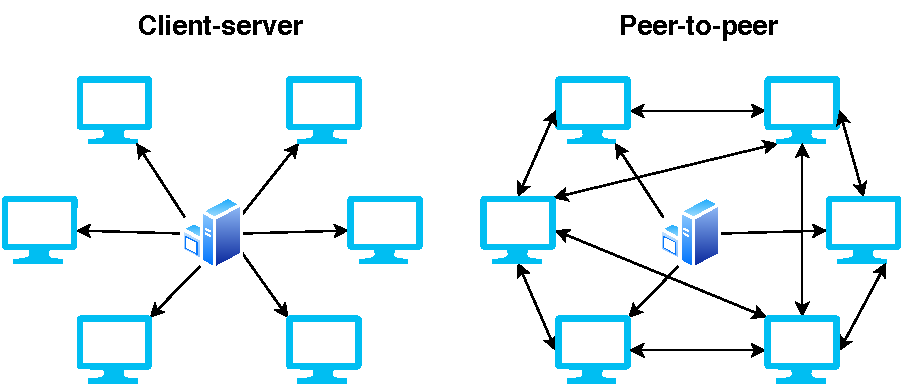
\includegraphics[width=0.6\linewidth]{fig/p2p.pdf}
		\caption{客户端-服务器端网络和对等网络示意图}
		\label{fig:p2p}
	\end{figure}
	
	而比特洪流(BitTorrent, BT)协议\cite{wiki_bt}作为去中心化的快速的文件共享、传输协议,在对等网络中占据十分重要的地位。
	英国网络分析公司CacheLogic的调查指出,BitTorrent占据了互联网上约35\%的流量,并且有数亿用户每天都在使用\cite{internet_traffic}。
	大量的应用都采用了BitTorrent协议,如迅雷\cite{xunlei}和$\mu$Torrent\cite{utorrent}运用BT协议进行文件传输,Facebook\cite{facebook}和Twitter\cite{twitter}都采用BT协议进行内容分发,Amazon S3则内置了BT协议进行分布式的文件存储。
	由此可以看出BitTorrent协议的重要性,故本文将对BT协议进行详细阐述,同时给出其实现方法供后人参考。
	
	\section{BitTorrent协议}
	BitTorrent协议是一个文件分发协议,它使用URL来定位内容并且能够与互联网进行无缝衔接。
	它相比纯HTTP的好处在于当同个文件的多个下载同时进行时,下载者可以通过上传自己已获得的部分文件供其他人下载,从而实现快速的大文件传输。
	
	BitTorrent协议最早由Bram Cohen于2001年提出,最初只能连接两个实体,传输速度也十分受限\cite{bt_ppt}。
	随着互联网的不断发展,BitTorrent协议也不断更新及完善,现在已能够实现大规模应用,并且充分利用网络带宽,实现快速的文件传输。
	本文将针对2017年的协议规范(BitTorrent Enhancement Proposals, BEPs)\cite{bt_org}进行阐述\footnote{注意这是BT协议公开的最新版本},先介绍BitTorrent的基本概念,然后逐一阐述每一个环节的内容,再对完整的文件分享流程进行叙述,最后对具体的算法进行介绍。
	
	\subsection{概述}
	在BitTorrent协议中主要有三方面的内容,首先是以B编码的元信息文件(见第\ref{sub:bencoding}节和第\ref{sub:metainfo}节),其次是参与协议工作的各类实体。
	
	对等实体可以分为播种者(seeder)和吸血者(leecher)。
	播种者即将自己的文件做成种子,然后对外进行分享。
	而吸血者仅仅下载别人的文件,而不自己做种,其他人将无法从它这里获得好处。
	
	还有一种实体是追踪者(tracker),它记录某个文件在哪些播种者中存在副本,并将这些信息告知需要下载文件的对等实体。
	
	关于对等实体的内容见第\ref{sub:peer}节,追踪者的内容见第\ref{sub:tracker}节,BitTorrent协议的具体流程见第\ref{sub:share}节,具体协议内的算法见第\ref{sub:peer_alg}节和第\ref{sub:sel_alg}节。
	
	\subsection{B编码}
	\label{sub:bencoding}
	B编码(Bencoding)是一种数据紧密存储的方式,具体的格式如表\ref{tab:bencoding}所示。
	注意任意两项之间没有任何空格,仅仅通过不同的格式区分。
	列表的内容可以是任意不同类型的组合,即列表内可以嵌套列表也可以包含字符串或字典。
	
	\begin{table}[htbp]
		\caption{B编码的格式}
		\label{tab:bencoding}
		\centering
		\begin{tabular}{|c|c|c|}\hline
			\textbf{类型} & \textbf{格式} & \textbf{例子}\\\hline
			字符串 & \verb'<length>:<data>' & \verb'7:network'\\\hline
			整数 & \verb'i<integer>e' & \verb'i3e'\\\hline
			列表 & \verb'l<contents>e' & \verb'l8:advanced7:networke'\\\hline
			字典 & \verb'd<keys><values>e' & \verb'd3:onei1e3:twoi2e5:threei3e4:fouri4ee'\\\hline
		\end{tabular}
	\end{table}
	
	\subsection{元信息文件}
	\label{sub:metainfo}
	元信息(metainfo)文件,即我们常见的\verb'.torrent'格式的文件或种子文件,用B编码存储,包含了以下信息:
	\begin{itemize}
		\item 公告(announce):追踪者的url地址,详情见第\ref{sub:share}节。
		\item 信息(info):一个字典,其中键值如下,都采用UTF-8编码。
		\begin{itemize}
			\item 文件名称(name):一个字符串。如果涉及多个文件或文件夹,则在信息中还包含路径名称(path)。
			\item 片段长度(piece length):每一个片段的字节数。为了传输方便,BitTorrent协议将文件分为等大的片段(除了最后一段)。每一个文件片段的长度通常是2的指数次幂,目前默认为$2^{18}=256$字节。
			\item 片段(piece):每20个字节代表一个片段的SHA1哈希值,总长度总为20的倍数。
			\item 其他可选项:如公告列表、创建日期、创建者、评论等。
		\end{itemize}
	\end{itemize}
	
	如图\ref{fig:test_torrent}所示,元信息文件的格式还是比较清晰的。
	红色框标注的部分为键的名称,后面紧跟的为键值。
	\begin{figure}[htbp]
		\centering
		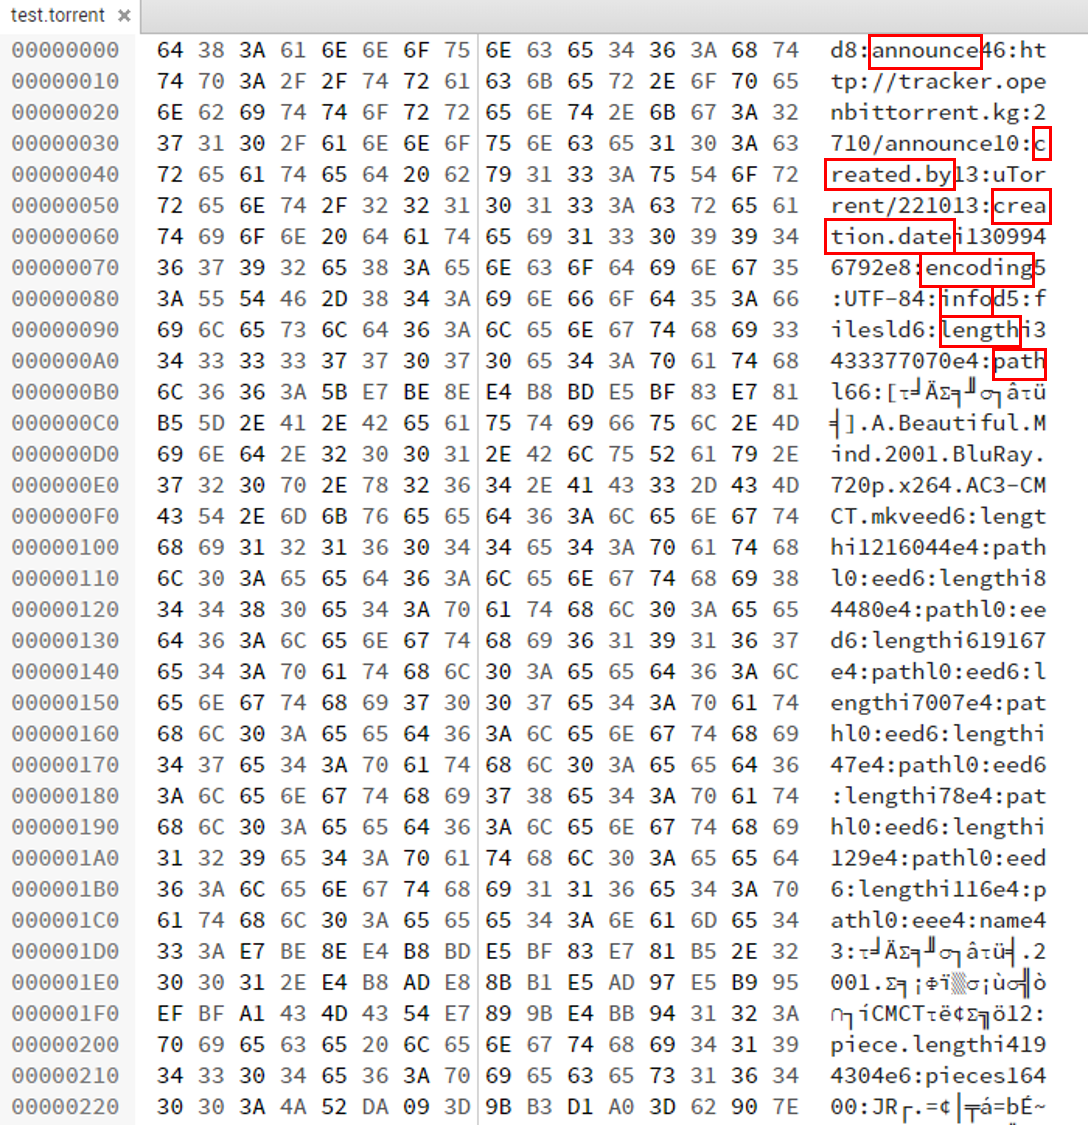
\includegraphics[width=0.6\linewidth]{fig/test_torrent_new.PNG}
		\caption{Torrent测试文件}
		\label{fig:test_torrent}
	\end{figure}
	
	\subsection{对等实体互连协议}
	\label{sub:peer}
	对等实体互连协议(peer wire protocol)构建在TCP或$\mu$TP协议\cite{bt_utp}上,其连接都是全双工的。
	
	当一个对等实体下载完一个片段并查验其哈希值匹配后,它将对所有实体公告它已经拥有该片段,从而其他实体可以从它这里下载该片段。
	
	对等实体连接两端都包含以下两种不同的状态,用两个二进制位存储:
	\begin{itemize}
		\item 阻塞(choked):若某一客户端被远端的播种者阻塞,则该客户端无法从该播种者处获取片段。
		\item 感兴趣(interested):若某一客户端对远端的播种者的片段感兴趣,则该客户端将在未阻塞时从该播种者处获取片段。
	\end{itemize}
	数据传输仅仅发生在一方感兴趣,另一方没有阻塞时。
	
	对等实体之间建立连接需要进行握手确认,其握手信号如下所示。
	\begin{center}
		\verb'<pstrlen><pstr><reserved><info_hash><peer_id>'
	\end{center}
	各字段含义如表\ref{tab:client_handshake}所示。
	\begin{table}[htbp]
		\caption{对等实体间握手信号字段含义}
		\label{tab:client_handshake}
		\centering
		\begin{tabular}{|c|c|}\hline
			\textbf{字段名} & \textbf{描述}\\\hline
			\verb'pstrlen' & \verb'pstr'的长度,目前设为19\\\hline
			\verb'pstr' & \begin{tabular}{c}协议标识符字符串\\目前用\verb'"BitTorrent protocol"'作为标识\end{tabular}\\\hline
			\verb'reserved' & 8个保留字节\\\hline
			\verb'info_hash' & 元信息文件中信息键值的20字节SHA1哈希编码\\\hline
			\verb'peer_id' & 每个实体独立的ID编号,20字节字符串\\\hline
		\end{tabular}
	\end{table}
	
	\subsection{追踪者传输协议}
	\label{sub:tracker}
	追踪者一般采用HTTP协议,分为请求和回复两个阶段。
	
	请求阶段,对等实体通过HTTP GET指令向追踪者发送请求,其中GET的参数如表\ref{tab:request}所示。
	\begin{table}[htbp]
		\caption{追踪者HTTP协议GET请求}
		\label{tab:request}
		\centering
		\begin{tabular}{|c|c|}\hline
			\textbf{参数名} & \textbf{描述}\\\hline
			\verb'info_hash' & 元信息文件中的20字节SHA1哈希值\\\hline
			\verb'peer_id' & 20字节客户端ID字符串\\\hline
			\verb'port' & 客户端监听的端口号,默认保留端口为6881-6889\\\hline
			\verb'uploaded' & 当前已上传总量,以十进制ASCII编码\\\hline
			\verb'downloaded' & 当前已下载总量,以十进制ASCII编码\\\hline
			\verb'numwant' & 请求对等实体数目,默认为50\\\hline
		\end{tabular}
	\end{table}
	
	回复阶段,追踪者通过HTTP协议向对等实体回复信息,具体参数如表\ref{tab:respond}所示。
	\begin{table}[htbp]
		\caption{追踪者HTTP协议回复}
		\label{tab:respond}
		\centering
		\begin{tabular}{|c|c|}\hline
			\textbf{参数名} & \textbf{描述}\\\hline
			\verb'complete' & 播种者的数目\\\hline
			\verb'incomplete' & 非播种者的数目\\\hline
			\verb'peers' & 一个字典,包括对等实体ID、IP地址及端口号\\\hline
		\end{tabular}
	\end{table}
	
	与追踪者的握手信号如表\ref{tab:tracker_handshake}所示。
	其中\verb'Bitfield'同样用来指代当前已经被成功下载的片段编号,需要在握手信号已经完成,还未进行其他消息发送之前进行告知。
	\verb'X'代表位域长,位域的最高位代表片段0。
	而\verb'Have'则在建立连接后用来指代当前已经被成功下载的片段编号,同样需要发送给追踪者,方便获取新的播种者名单。
	\begin{table}[htbp]
		\caption{追踪者握手信号含义}
		\label{tab:tracker_handshake}
		\centering
		\begin{tabular}{|c|c|c|c|}\hline
			\textbf{握手信号} & \verb'<length prefix>' & \verb'<message ID>' & \verb'<payload>'\\\hline
			Keep-alive & 0000 & 0 & 无\\\hline
			Choke & 0001 & 0 & 无\\\hline
			Unchoke & 0001 & 1 & 无\\\hline
			Interested & 0001 & 2 & 无\\\hline
			Not-interested & 0001 & 3 & 无\\\hline
			Have & 0005 & 4 & 片段编号\\\hline
			Bitfield & 0001+X & 5 & 位域\\\hline
			Request & 0013 & 6 & \verb'<index><begin><length>'\\\hline
			Piece & 0009+X & 7 & \verb'<index><begin><block>'\\\hline
			Cancel & 0013 & 8 & \verb'<index><begin><length>'\\\hline
			port & 0003 & 9 & \verb'<listen-port>'\\\hline
		\end{tabular}
	\end{table}
	
	由于HTTP协议基于TCP协议,需要连接始终保持开启,同时导致大量数据开销,故为了减少开销,BitTorrent的追踪者协议也可以基于UDP协议进行,这在BEP15\cite{bt_udp}中进行了规定。
	
	另一方面,由于单一的追踪者已无法满足这么多对等实体的需求,故现在更多采用分布式稀疏哈希表(Distributed sloppy Hash Table, DHT)用来存储对等实体的通信信息。
	每个对等实体都将成为一个追踪者,这在BEP5\cite{bt_dht}中进行了规定。
	
	\subsection{文件共享机理}
	\label{sub:share}
	BitTorrent协议完整的操作流程如图\ref{fig:overview}所示。
	
	\begin{figure}[htbp]
		\centering
		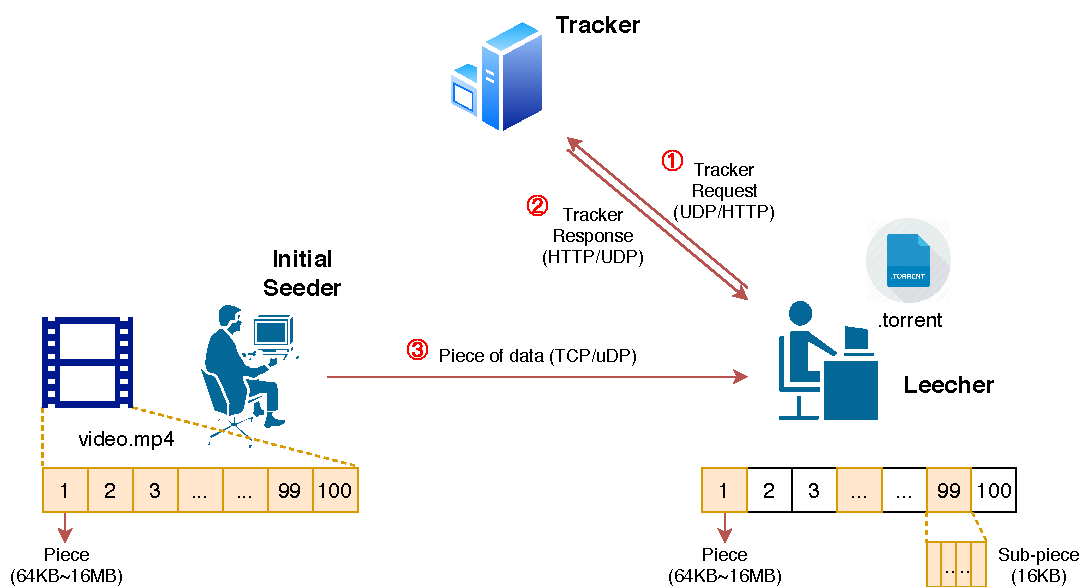
\includegraphics[width=0.7\linewidth]{fig/BitTorrent-BitTorrent.pdf}
		\caption{BitTorrent协议完整流程}
		\label{fig:overview}
	\end{figure}
	
	初始的播种者将要传输的文件分割为很多片段,每个片段的长度取值可以从64KB到16MB。
	吸血者从元信息文件的\verb'announce'键值中获取追踪者的信息,然后通过HTTP或UDP的方式与追踪者建立连接。
	追踪者将播种者的IP地址、端口号等信息回传给吸血者。
	吸血者根据对应的信息通过TCP或$\mu$DP方式,与播种者建立连接,并逐次下载对应片段。
	每个片段又可划分为很多个子片段,其中16KB的子片段为最小传输单位。
	当吸血者获取了所有片段并依序整合后,传输结束。
	
	而吸血者在获取了部分片段后可以转变成播种者,同样共享资源给其他吸血者下载。
	如图\ref{fig:overview-2}所示,新的吸血者同样从追踪者处获取播种者名单。
	追随者默认会返回50个随机的播种者,吸血者将并行地从这些播种者处获取缺失的片段,直到所有片段都收集齐为止。
	因此BitTorrent协议具有更多播种者,更多资源副本,下载速度更快的特点。
	
	注意,由于种子文件较小,故一般可以通过搜索引擎或专门的种子服务器得到,由于不是本文的重点,故图中未给出种子传播的途径。
	\begin{figure}[htbp]
		\centering
		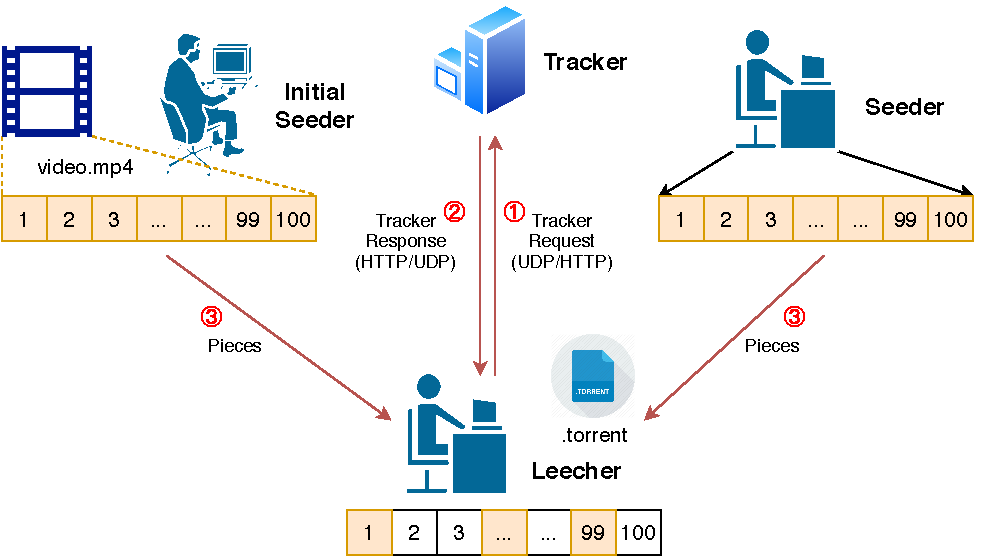
\includegraphics[width=0.7\linewidth]{fig/BitTorrent-BitTorrent-2.pdf}
		\caption{BitTorrent协议完整流程(多个播种者)}
		\label{fig:overview-2}
	\end{figure}
	
	\subsection{对等实体选择算法}
	\label{sub:peer_alg}
	对等实体选择策略用来决定从哪里下载对应片段,目前BitTorrent协议主要采用以下几种算法\cite{survey_bt}:
	\begin{itemize}
		\item 以牙还牙(Tit-for-tat, TFT)策略:一个对等实体更倾向于将其片段分享给那些提供给它更大下载速率的实体。这个策略大幅提升了BitTorrent协议的性能,有效避免搭便车的实体(free-rider),即只下载不上传。
		\item 最优非阻塞:每隔30秒,一个对等实体会随机将它的邻居实体取消阻塞,而无关其上传速率。这能有效发现一些上传速度更快的对等实体。
		\item 反冷落(anti-snubbing)算法:如果一个实体注意到隔了一段时间它都没有从某一实体处获得片段,则该实体会认为被对方冷落了,并采取反制措施,不再向其上传片段。
		\item 只上传算法:一旦一个对等实体完成整个文件的下载,它将变成播种者。因为播种者没有其他东西要下载,因此无法基于下载速率选择最好的对等实体。相反地,播种者会更倾向于选择与有更优上传速率的实体进行分享。
	\end{itemize}
	
	\subsection{片段选择算法}
	\label{sub:sel_alg}
	由于吸血者需要从播种者处获取文件片段(piece),最后再一并整合,故获取哪一个片段是需要考虑的问题,常见的有以下几种算法:
	\begin{itemize}
		\item 严格优先:对等实体只关注于当前下载的片段,先将当前片段的所有子片段下载完,才下载其他片段。这可以保证自己有完整的片段可以与其他实体进行交易。
		\item 稀少优先:这是一般的情况,对于在所有对等实体中最缺失的片段,应该最先下载。这可以保证最常见的片段留到最后才进行下载。
		\item 随机优先:同字面意思,随机选取片段进行下载。
		\item 游戏终止模式(End game mode):为避免获取最后几个片段造成的延迟,对等实体将向其他所有实体发送请求。而一旦片段获得,则应发送\verb'cancel'消息给不必要的对等实体,防止带宽浪费。
	\end{itemize}
	
	\section{实现细节}
	在本次研究过程中,我们设计实现了一个简化的BT协议。并且独立地使用C++语言,基于前面几次套接字实验的经验,编写了服务器和客户端程序。程序实现的基本功能有:创建、解析种子文件与下载、校验对应文件。接下来分协议(\ref{sub:bt}节),服务器(\ref{sub:server}节),客户端(\ref{sub:client}节)三个部分介绍。
	\subsection{BT协议}
	\label{sub:bt}
	我们的BT协议是基于标准的BT协议简化而来,保留了BT协议中的必选字段\ref{tab:btfile},删除了部分目前没有实现的字段,目前支持多个用户在局域网内进行单文件分享。
	
	一个标准的BT种子文件(.torrent)格式如图\ref{fig:torrent},实现结果如图\ref{fig:torrentfile}。其中服务器地址和片段大小由用户在制作种子时输入,文件长度以及每个片段的SHA1哈希值由程序计算得来。
	
	一个典型的,基于BT协议的,分享文件的过程为:
	\begin{enumerate}
		\item 文件拥有者启动客户端,用客户端制作种子文件,然后向服务器发出通知,告诉服务器文件名、IP地址和监听的端口号。
		\item  其他用户通过各种手段(种子分享网站、云盘或U盘)得到种子之后运行客户端,解析种子文件信息,根据种子文件中存储的信息(announce和name)向服务器索要文件拥有者的信息(IP地址和端口号)。
		\item 下载者和文件拥有者(可能有多个)建立连接,下载文件
		\item 下载完所有块之后,对每一块进行SHA1哈希校验,如果都成功则接受,否则报告错误并退出下载
		\item 下载完成之后,转变为文件的拥有者,并通知服务器。
	\end{enumerate}
	
	
	这里,我们将服务器与客户端间的通信机制设置为如下格式。
	\begin{center}
		\verb'<peer_num> <IP1> <Port1> <IP2> <Port2> ...'
	\end{center}
	客户端可发布三种命令。0号命令用于发布文件信息,1号命令用于获取文件拥有者列表,2号命令表示不再对外分享文件并退出连接。服务器则只会对1号命令回复有效信息,即一个文件拥有者列表。
	
	\begin{table}[htbp]
		\caption{Tracker与node间通信机制}
		\label{tab:r}
		\centering
		\begin{tabular}{|c|c|c|}\hline
			\textbf{指令号} & \textbf{指令格式} & \textbf{描述}\\\hline
			\verb'0' & \verb'<filename> <port>' & 用于接受连接的数据端口\\\hline
			\verb'1' & \verb'<filename>'& 需要下载的文件名\\\hline
			\verb'2' & \verb'none' & 退出连接\\\hline
		\end{tabular}
	\end{table}
	
	种子文件结构如下所示。
\begin{lstlisting}
{
    announce: `服务器地址(字符串)'
    info:{
        length: `文件长度(整数)'
        name: `文件名(字符串)'
        piece_length: `每块字节数(整数)'
        pieces: `块校验码(字符串)'
    }
}
\end{lstlisting}
	\begin{table}[htbp]
		\caption{torrent文件各个字段含义}
		\label{tab:btfile}
		\centering
		\begin{tabular}{|c|c|}\hline
			\textbf{字段名} & \textbf{描述}\\\hline
			\verb'announce' & 服务器地址\\\hline
			\verb'info' & 目标文件信息,包含以下内容 \\\hline
			\verb'length' & 目标文件长度\\\hline
			\verb'name' & 目标文件名\\\hline
			\verb'piece_length' & 片段大小 \\\hline
			\verb'pieces' & 每个片段的20个字节的SHA1哈希值 \\\hline
		\end{tabular}
	\end{table}
	\begin{figure}[htbp]
		\centering
		\subfigure[discre.torrent]{
			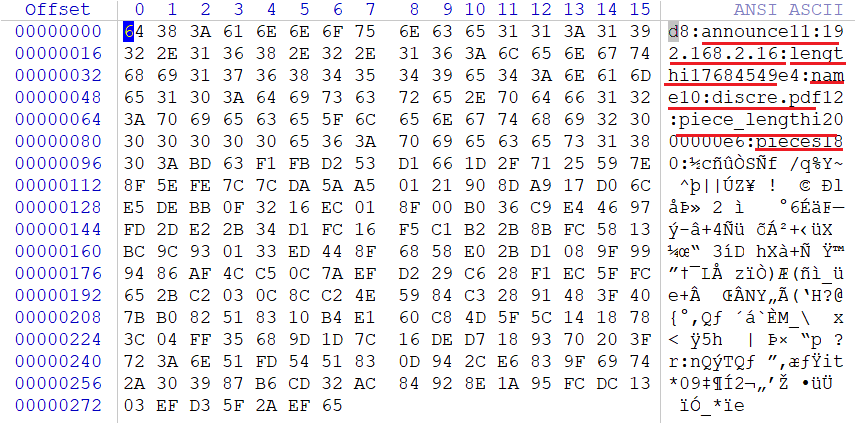
\includegraphics[width=0.6\linewidth]{fig/discre.png}	
		}
		\subfigure[inte.torrent]{
			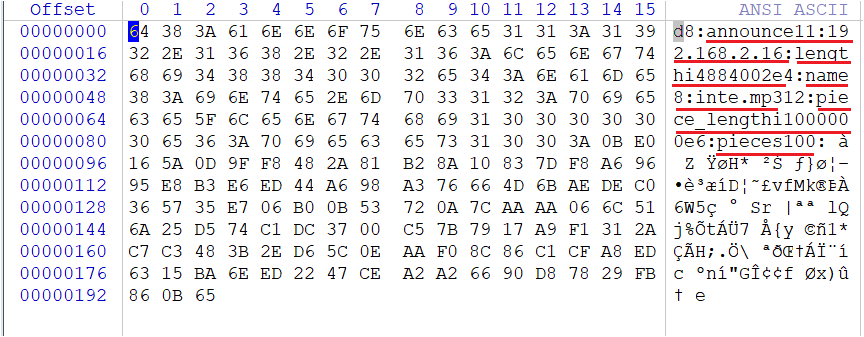
\includegraphics[width=0.6\linewidth]{fig/inte.png}
		}
		\caption{客户端做的种子}
		\label{fig:torrentfile}
	\end{figure}

	\subsection{服务器}
	\label{sub:server}
	这里实现了一个简化版的Tracker服务器,用于维护与发布当前网络中的种子信息。服务器与客户端间的通信使用TCP协议,而客户端会设置一个特殊的控制端口专用于传达指令。
	
	一个完整的通信流程如下:
	\begin{enumerate}
		\item 第一个文件持有客户端会与服务器建立连接并告知服务器自己拥有的文件名,IP地址与数据端口号,服务器会将信息登记存储。
		\item 当一个客户端需要下载这个文件时,会根据种子文件获取服务器的IP地址,与服务器建立连接,并告知服务器自己需要的文件;服务器将依据文件名返回一个文件拥有者的列表。
		\item 当一个文件拥有者退出连接时,服务器会将记录中与其IP地址匹配的表项全部清除。
	\end{enumerate}

	\subsection{客户端}
	\label{sub:client}
	客户端具有并行处理功能,启动之后客户端同时并行执行两个线程:主线程负责读取并执行用户命令;一个\verb|upload|线程等待其他客户端的连接,准备传输文件。
	
	客户端目前支持制作种子与下载文件功能。
	
	制作种子时,由用户输入目标文件名、tracker服务器地址和种子文件分块大小。客户端将目标文件分块读取并为每一块生成20字节的SHA1哈希校验码存在种子文件中。创建完种子之后,客户端向服务器发布消息,包括文件名和\verb|upload|线程监听的端口号(默认为50520)。
	
	下载文件时,客户端首先打开种子文件并解析其中的信息。然后根据\verb|announce|字段连接服务器,根据\verb|name|字段向服务器询问文件拥有者的信息。服务器返回一个文件拥有者的列表给客户端。如果有n个拥有者,客户端就会尽量将文件分为n份(每一份都是块大小的整数倍),然后启动n个\verb|download_t|子线程向每个拥有者索要对应的文件块。主线程等待每个子线程下载完毕之后,按顺序读取各个临时文件,存储到最终下载的目标文件中,每读一块数据进行一次SHA1哈希校验,如果和种子文件中存储的哈希值相同则接受,否则报错并退出下载。将临时文件合并完之后,删除临时文件。下载完毕之后,客户端就转变为了文件的拥有者,向服务器发出通知,告知服务器文件名和监听的端口号。之后就可以向其他客户端发送该文件。
	
	
	下面的内容详细介绍了客户端的各个模块具体工作原理。
	\subsubsection{文件下载与上传}
	文件的下载与上传是客户端的核心功能,客户端在启动之后就立即开启\verb|upload|线程,随时准备接受其他客户端的连接,向其他客户端发送文件。而每当用户输入下载文件的命令时,客户端就进入\verb|download|函数,下载对应的文件。
	
	\paragraph{upload}
	类似于聊天程序客户端,每收到一个连接请求,\verb|upload|线程就启动一个\verb|upload_t|子线程负责通信。
\begin{lstlisting}
void upload()
{
	SOCKET msock, sock;
	struct sockaddr_in sin, fsin;
	int alen = sizeof(struct sockaddr_in);

	msock = socket(PF_INET, SOCK_STREAM, IPPROTO_TCP);

	memset(&sin, 0, sizeof(sin));
	sin.sin_family = AF_INET;
	sin.sin_addr.s_addr = INADDR_ANY;
	sin.sin_port = htons((u_short)stoi(lis_port));
	bind(msock, (struct sockaddr *)&sin, sizeof(sin));

	listen(msock, 5);

	while (true)
	{
		sock = accept(msock, (struct sockaddr *)&fsin, &alen);
		mu.lock();
		cout << "`收到'" << inet_ntoa(fsin.sin_addr) << "`的连接请求!'" << endl;
		mu.unlock();
		thread temp(upload_t, sock);
		temp.detach();
	}

	return;
}
\end{lstlisting}

	\paragraph{upload\_t}
	\verb|upload_t|函数实现如下。upload函数从下载者那里接受要上传的文件名、文件起始位置和字节数。然后打开对应的文件,将文件指针移动到指定位置,读取指定数量的字节并发送。
\begin{lstlisting}
void upload_t(SOCKET sock)
{
	char buff[bufflen];
	//`文件名'
	int cc = recv(sock, buff, bufflen, 0);
	buff[cc] = 0;
	ifstream myifs(string(buff), ios::binary);
	//`send只起同步作用'
	send(sock, "y", 1, 0);
	//`起始位置'
	cc = recv(sock, buff, bufflen, 0);
	buff[cc] = 0;
	int start = stoi(string(buff));
	send(sock, "y", 1, 0);
	//`字节数'
	cc = recv(sock, buff, bufflen, 0);
	buff[cc] = 0;
	int num = stoi(string(buff));
	//`移动文件指针'
	myifs.seekg(start, ios::beg);
	mu.lock();
	cout << "`正在发送文件!'" << endl;
	mu.unlock();
	while (!myifs.eof() && num > 0)
	{
		myifs.read(buff, min(bufflen, num));
		send(sock, buff, myifs.gcount(), 0);
		num -= myifs.gcount();
	}
	myifs.close();
	mu.lock();
	cout << "`文件发送成功!'" << endl;
	mu.unlock();

	return;
}
\end{lstlisting}
	
	\paragraph{download}
	download函数首先根据种子文件的信息(存储在结构体tf中)连接服务器(tf.announce),向服务器询问指定文件(tf.name)的拥有者。服务器返回文件拥有者的列表,其中包含IP地址和端口号。这部分的代码如下。
\begin{lstlisting}
struct sockaddr_in sin;
SOCKET sock;

char buff[bufflen];

sock = socket(PF_INET, SOCK_STREAM, IPPROTO_TCP);

memset(&sin, 0, sizeof(sin));
sin.sin_family = AF_INET;
sin.sin_addr.s_addr = inet_addr(tf.announce.c_str());
sin.sin_port = htons((u_short)stoi(server_port));
int ret = connect(sock, (struct sockaddr*)&sin, sizeof(sin));

if (ret == 0)
{
	send(sock, "1", 1, 0);
	recv(sock, buff, bufflen, 0);
	send(sock, tf.name.c_str(), tf.name.length(), 0);
	int cc = recv(sock, buff, bufflen, 0);
	buff[cc] = 0;
	map<string, string> target;
	//`解析返回的文件拥有者列表'
	istringstream ifs(buff);
	int n;
	ifs >> n;
	mu.lock();
	cout << "`找到'" << n << "`个拥有者!'" << endl;
	mu.unlock();
	// ... continued
\end{lstlisting}
	
	客户端解析服务器返回的列表之后,会根据目前文件拥有者的数目决定开启几个线程下载、每个线程需要下载的块数目。
	
	假如目前有n个文件拥有者,文件有m块,那么客户端最多会启动n个线程下载,每个线程最多下载$\lceil \frac{m}{n}\rceil$块。
	\begin{itemize}
		\item 假设目标文件有8块,目前有3个拥有者。那么客户端启动3个线程,分别下载3,3,2块。
		\item 假设目标文件有2块,目前有3个拥有者。那么客户端会启动2个线程,分别下载1,1块。
	\end{itemize}
	
	对于每个文件拥有者,客户端启动一个\verb|download_t|子线程与之通信,\verb|download_t|函数需要文件名,IP地址,端口号,起始下载位置,下载字节数和序号作为参数。
\begin{lstlisting}
for (int i = 0; i < n; i++)
{
	string ip, port;
	ifs >> ip >> port;
	target[ip] = port;
}
//`计算文件的总块数'
int piece_num = (tf.length + tf.piece_length - 1) / tf.piece_length;
//`计算每个线程应该下载的块数'
int task_num = (piece_num + n - 1) / n;
//`一个线程向一个拥有者索要'
int index = 0;
int num = tf.length;
vector<thread*> t_pool;
for (auto item : target)
{
	/*`最后一个可能会有不足'*/
	t_pool.push_back(new thread(download_t, item.first, item.second, tf.name, index*task_num*tf.piece_length,
		min(task_num*tf.piece_length, num), index));
	++index;
	num -= task_num * tf.piece_length;
	if (num <= 0)
		break;
}

for (auto item : t_pool)
{
	item->join();
	delete item;
}
\end{lstlisting}
	
	之后,主线程等待所有子线程执行完毕后,将所有子线程下载的临时文件(*index.temp)按顺序读取。每读取一块数据,就进行一次SHA1哈希校验,和种子文件中存储的哈希值进行比较,如果校验失败则报错并退出下载;否则将数据写入到最终的目标文件中。
	
	所有校验完毕之后,文件就下载成功了。客户端会通知服务器,告诉服务器自己拥有的文件、IP地址和监听的端口号。
\begin{lstlisting}
for (int i = 0, j = 0; i < index; i++)
{
	string tempname = tf.name + to_string(i) + ".temp";
	ifstream tempifs(tempname, ios::binary);
	cout << "`正在合并临时文件'" << i << "`!'" << endl;
	while (!tempifs.eof())
	{
		tempifs.read(tempbuff, tf.piece_length);
		int a = tempifs.gcount();
		if (a <= 0)
			break;
		tempbuff[a] = 0;
		string tem(tempbuff);
		//`对收到的文件块进行hash校验'
		if (tf.pieces[j++] != SHA1(tempbuff, tempifs.gcount()))
		{
			cerr << "`校验失败!'\n";
			tempifs.close();
			myofs.clear();
			myofs.close();
			return;
		}
		myofs.write(tempbuff, tempifs.gcount());
	}
	tempifs.close();
	remove(tempname.c_str());
	cout << "`临时文件'" << i << "`合并成功!'" << endl;
}
myofs.close();
mu.lock();
cout << tf.name << "`下载成功!'" << endl;
mu.unlock();
//`通知服务器'
send(sock, "0", 1, 0);
recv(sock, buff, bufflen, 0);
send(sock, tf.name.c_str(), tf.name.size(), 0);
recv(sock, buff, bufflen, 0);
send(sock, lis_port.c_str(), lis_port.size(), 0);
\end{lstlisting}
	
	\subsubsection{SHA1哈希函数}
	在SHA1算法中,我们必须把原始消息转化成位串。消息必须进行补位,以使其长度在对512取模以后的余数是448。也就是说,(补位后的消息长度)\%512 = 448。即使长度已经满足对512取模后余数是448,补位也必须要进行。
	接着要将原始数据的长度补到已经进行了补位操作的消息后面。通常用一个64位的数据来表示原始消息的长度。
	
	在SHA1中我们使用一系列的函数。对于每组的512字节,分成16子组80次轮换计算摘要,具体细节这里不予赘述。
	
\begin{lstlisting}
std::string SHA1class::final()
{
	/* Total number of hashed bits */
	uint64_t total_bits = (transforms*BLOCK_BYTES + buffer.size()) * 8;

	/* Padding */
	buffer += (char)0x80;
	size_t orig_size = buffer.size();
	while (buffer.size() < BLOCK_BYTES)
	{
		buffer += (char)0x00;
	}

	uint32_t block[BLOCK_INTS];
	buffer_to_block(buffer, block);

	if (orig_size > BLOCK_BYTES - 8)
	{
		transform(digest, block, transforms);
		for (size_t i = 0; i < BLOCK_INTS - 2; i++)
		{
			block[i] = 0;
		}
	}

	/* Append total_bits, split this uint64_t into two uint32_t */
	block[BLOCK_INTS - 1] = (uint32_t)total_bits;
	block[BLOCK_INTS - 2] = (uint32_t)(total_bits >> 32);
	transform(digest, block, transforms);

	/* Hex std::string */
//    std::ostringstream result;
	std::string result;
	for (size_t i = 0; i < sizeof(digest) / sizeof(digest[0]); i++)
	{
		//        result << std::hex << std::setfill('0') << std::setw(8);
		//        result << digest[i];
		for (uint32_t j = 0, dig = digest[i]; j < 4; ++j, dig >>= 8)
			result += uint8_t(dig & 255);
	}

	/* Reset for next run */
	reset(digest, buffer, transforms);

	return result;
}
\end{lstlisting}
	
	\subsubsection{种子文件创建与读取}
	实验中的 BT种子结构比较简浅,只有一个字典嵌套若干字符串和一个列表。
	种子的解析和读取只需要额外书写几个读写字符串、整数、和列表的子函数
\begin{lstlisting}
string read_torrent_str(const char t[], int sz, int &i) {
	int strl = 0;
	assert(isdigit(t[i]));
	for (; i < sz && isdigit(t[i]); ++i)	strl = strl * 10 + t[i] - 48;
	assert(t[i++] == ':');
	assert(i + strl <= sz);
	//	string ret=t.substr(i, strl); i+=strl;
	string ret = "";
	for (int j = 0; j < strl; ++j, ++i) ret += t[i];
	return ret;
}

int read_torrent_int(const char t[], int sz, int &i) {
	assert(t[i++] == 'i');
	int num = 0, sgn = 1;
	if (t[i] == '-') sgn = -1, ++i;
	assert(isdigit(t[i]));
	for (; i < sz && isdigit(t[i]); ++i)num = num * 10 + t[i] - 48;
	assert(t[i++] == 'e');
	return num * sgn;
}

string make_torrent_int(int num) {
	string ret = "";
	int sgn = 1;
	if (num < 0)num = -num, sgn = -1;
	if (num == 0) ret = "0";
	else for (; num; num /= 10) ret += char(num % 10 + 48);
	reverse(ret.begin(), ret.end());
	if (sgn == -1) ret = "-" + ret;
	return "i" + ret + "e";
}

string make_torrent_str(string t) {
	return to_string(t.size()) + ":" + t;
}
\end{lstlisting}
	
	读取的函数如下
\begin{lstlisting}
torrent_file read_torrent(string filename) {
	//	ifstream fin(filename);
	//	ostringstream finbuf; finbuf<<fin.rdbuf();
	//	string s(finbuf.str());fin.close();
	//	torrent_file res;
	//	assert(s.front()=='d' && s.back()=='e');
	//	s=s.substr(1, s.size()-2);
	FILE *fin;
	fopen_s(&fin, filename.c_str(), "rb"); int filesz = 0;
	for (char tmpc; fread(&tmpc, 1, 1, fin); ++filesz);
	fclose(fin); fopen_s(&fin, filename.c_str(), "rb");
	char *s = new char[filesz + 1];
	fread(s, 1, filesz, fin); fclose(fin);
	assert(s[0] == 'd' && s[--filesz] == 'e');

	torrent_file res;
	for (int i = 1; i < filesz;) {
		string itname = read_torrent_str(s, filesz, i);

		if (itname == "announce") {
			res.announce = read_torrent_str(s, filesz, i);
		}
		else if (itname == "length") {
			res.length = read_torrent_int(s, filesz, i);
		}
		else if (itname == "name") {
			res.name = read_torrent_str(s, filesz, i);
		}
		else if (itname == "piece_length") {
			res.piece_length = read_torrent_int(s, filesz, i);
		}
		else if (itname == "pieces") {
			string totpiece = read_torrent_str(s, filesz, i);
			for (int j = 0; j < totpiece.size(); j += 20)
				res.pieces.push_back(totpiece.substr(j, 20));
		}
		else {
			fprintf(stderr, "Wrong on item name");
		}
	}

	delete[]s;
	return res;
}
\end{lstlisting}

	
	\section{实验结果}
		我们使用我们的BT程序做了多组文件传输实验,在实验中,我们利用一台路由器和五台电脑搭建了局域网,所有参与实验的电脑连接到局域网中并配置IP如表\ref{tab:equipment};实验过程中,我们使用了U盘分享种子文件,然后在不同的PC电脑上解析种子文件,下载对应的目标文件。最后的实验结果验证了协议与程序的正确性。
	\begin{table}[H]
		\caption{实验设备}
		\label{tab:equipment}
		\centering
		\begin{tabular}{|c|c|c|}\hline
			\textbf{设备名称} & \textbf{IP地址} &功能\\\hline
			\verb'PC1' & 192.168.2.1& 服务器\\\hline
			\verb'PC2' & 192.168.2.2& 客户端\\\hline
			\verb'PC3' & 192.168.2.3& 客户端\\\hline
			\verb'PC4' & 192.168.2.4& 客户端\\\hline
			\verb'PC5' & 192.168.2.5& 客户端\\\hline
		\end{tabular}
	\end{table}
	\subsection{1-1实验}
	我们首先进行了最简单的1个下载者和1个文件发布者之间的传输实验。PC1做服务器(图\ref{res:PC1_11})。PC2作为发布者(图\ref{res:PC2_11}),发布两份文件:discre.pdf和inte.mp3。制作的种子文件为:discre.torrent和inte.torrent。PC4解析两份种子文件,向PC2请求下载(图\ref{res:PC4_11})。1-1实验网络拓扑结构图如\ref{res:11}所示。最终下载的结果如图\ref{res:file},后面的几组实验同样是在下载这两份文件,因此不再做展示。

	\begin{figure}[H]
		\centering
		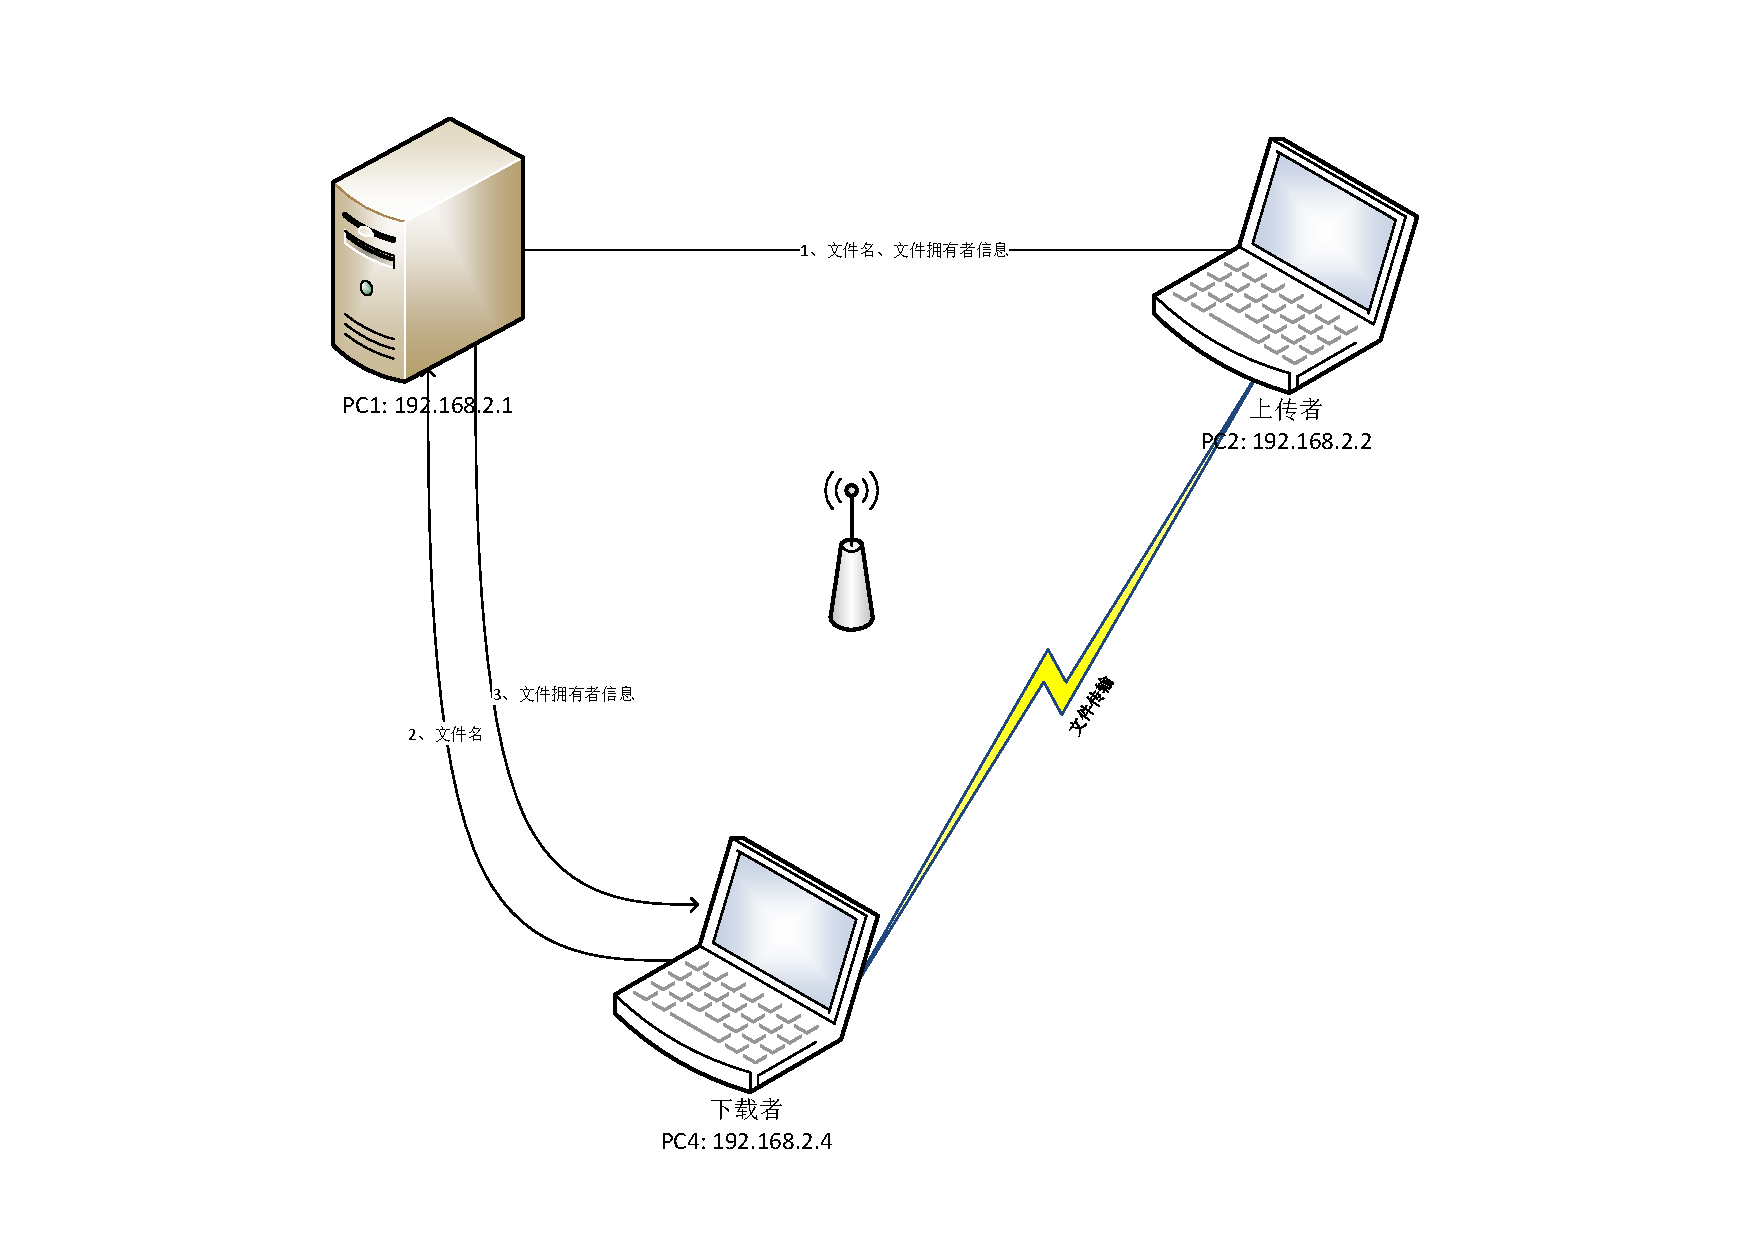
\includegraphics[width=0.6\linewidth]{fig/1-1.pdf}
		\caption{1-1实验\quad 网络拓扑结构图}
		\label{res:11}
	\end{figure}
	\begin{figure}[H]
		\centering
		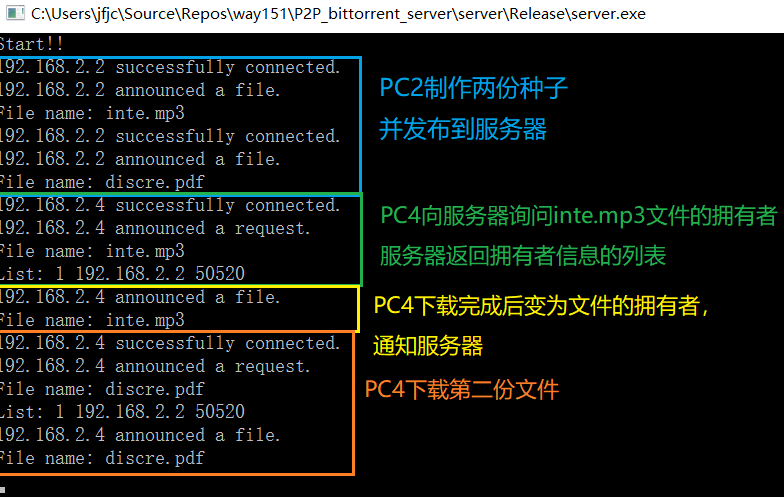
\includegraphics[width=0.6\linewidth]{fig/PC1_11.png}
		\caption{1-1实验\quad PC1作为服务器}
		\label{res:PC1_11}
	\end{figure}
	\begin{minipage}{0.5\linewidth}
	\begin{figure}[H]
		\centering
		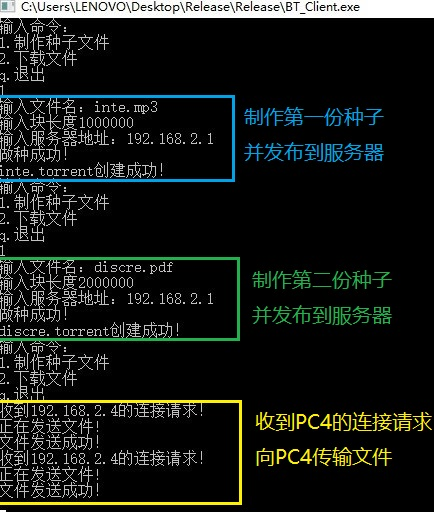
\includegraphics[width=\linewidth]{fig/PC2_11.jpg}
		\caption{1-1实验\quad PC2作为文件发布者}
		\label{res:PC2_11}
	\end{figure}
	\end{minipage}
	\begin{minipage}{0.5\linewidth}
	\begin{figure}[H]
		\centering
		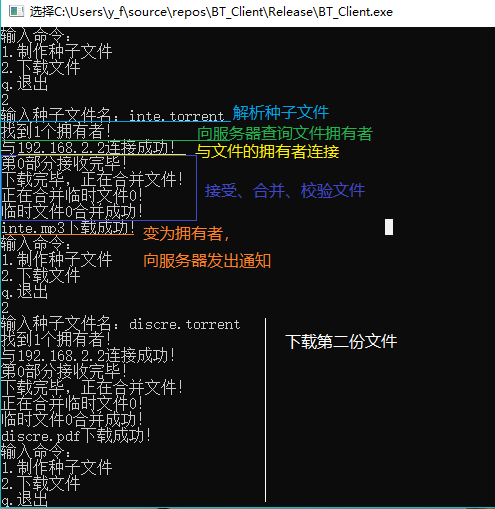
\includegraphics[width=\linewidth]{fig/PC4_11.png}
		\caption{1-1实验\quad PC4作为下载者}
		\label{res:PC4_11}
	\end{figure}
	\end{minipage}
	
	\begin{figure}[H]
		\centering
		\subfigure[PC2上的discre.pdf]{
			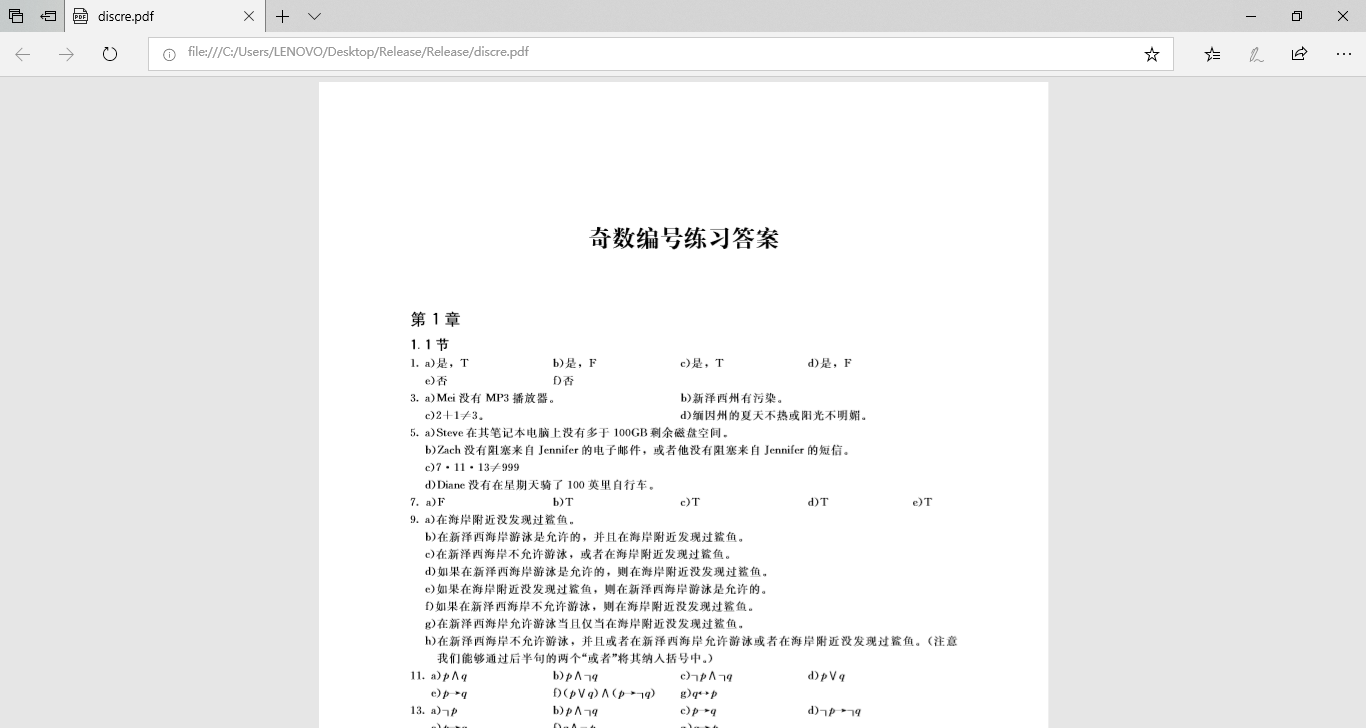
\includegraphics[width=0.45\linewidth]{fig/PC2_f1.png}
		}
		\subfigure[PC2上的inte.mp3]{
			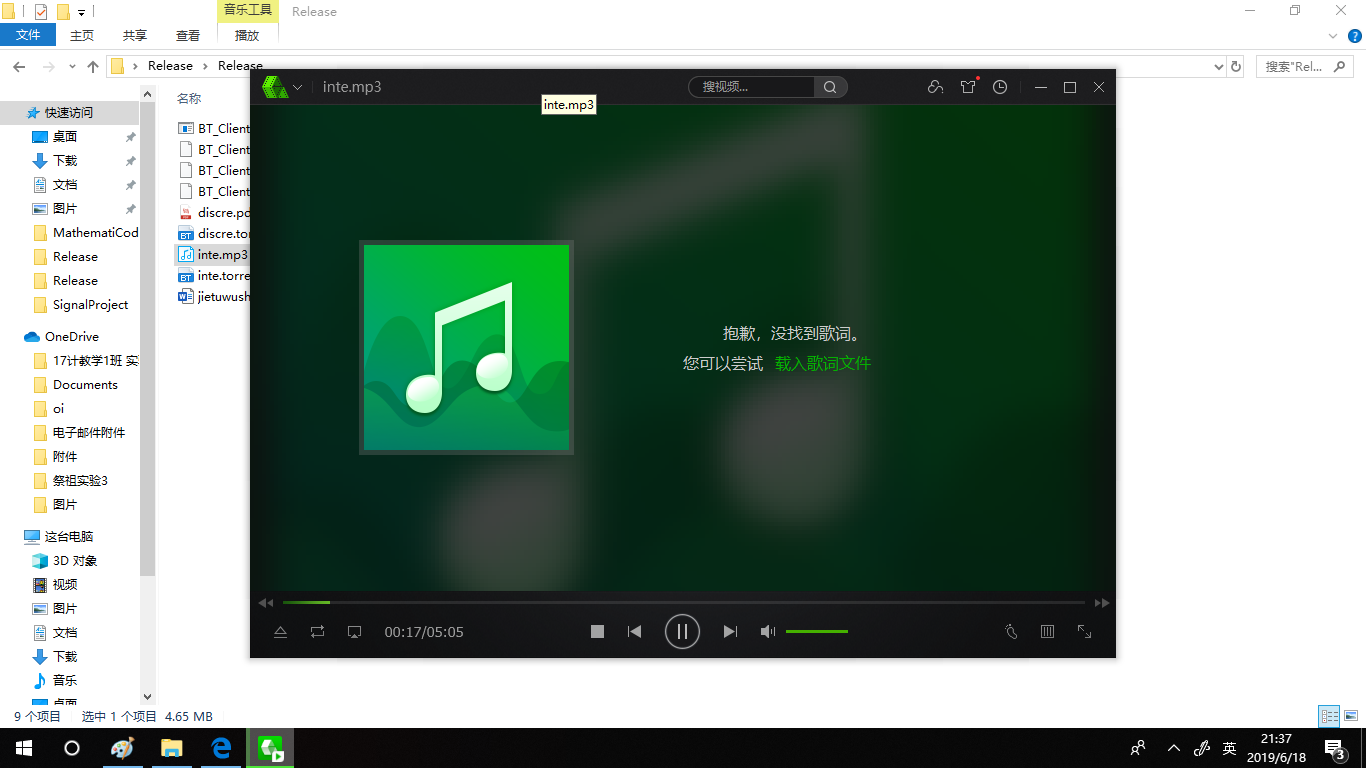
\includegraphics[width=0.45\linewidth]{fig/PC2_f2.png}
		}
		\subfigure[PC4接受的discre.pdf]{
			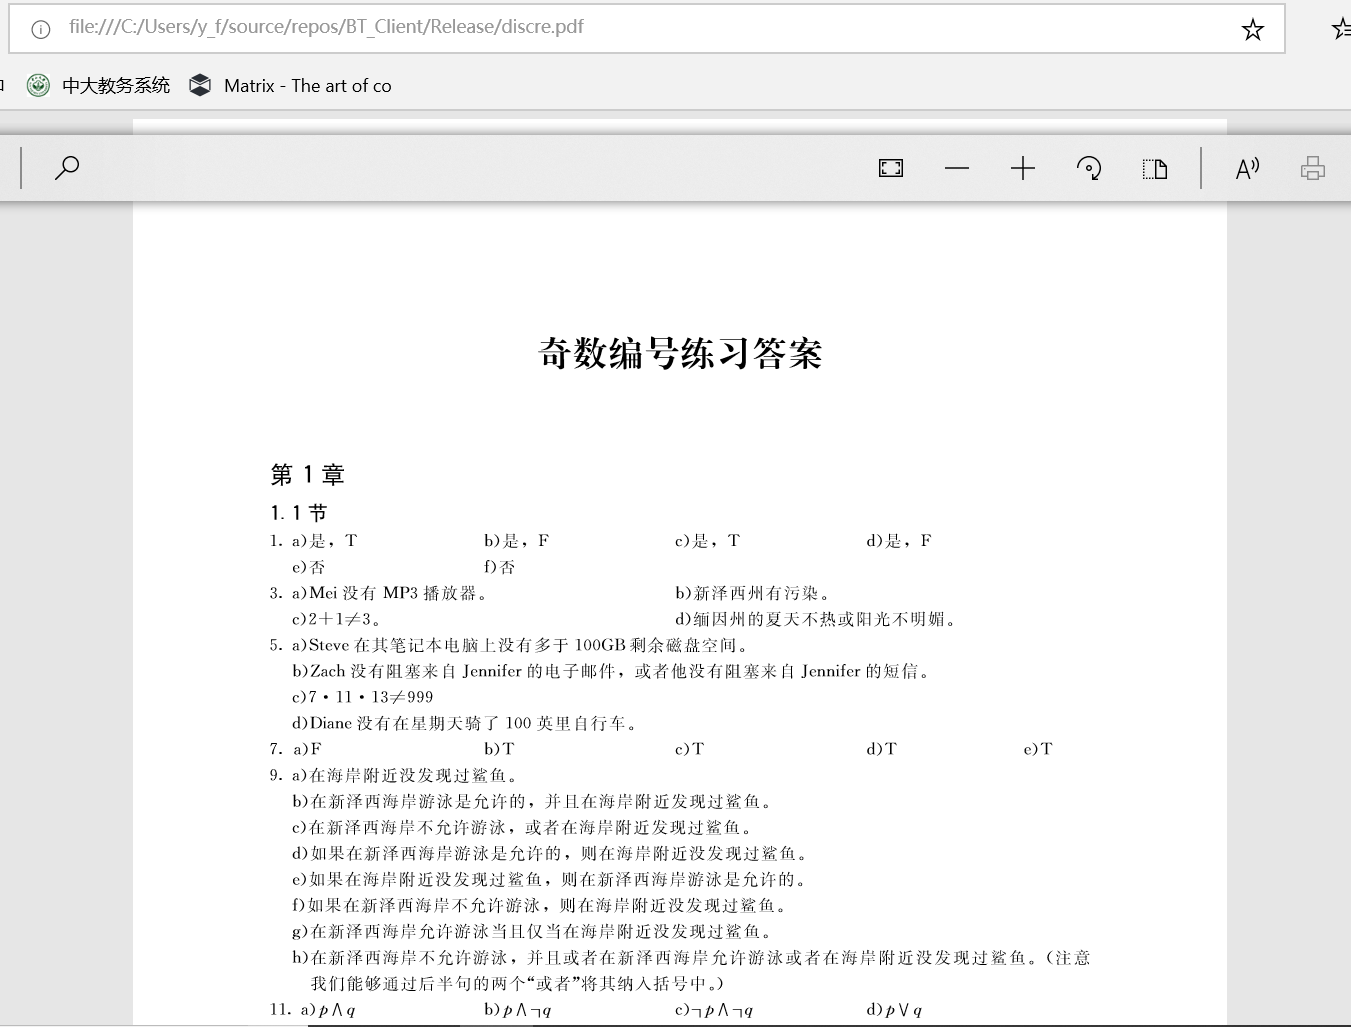
\includegraphics[width=0.45\linewidth]{fig/PC4_f1.png}
		}
		\subfigure[PC4接受的inte.mp3]{
			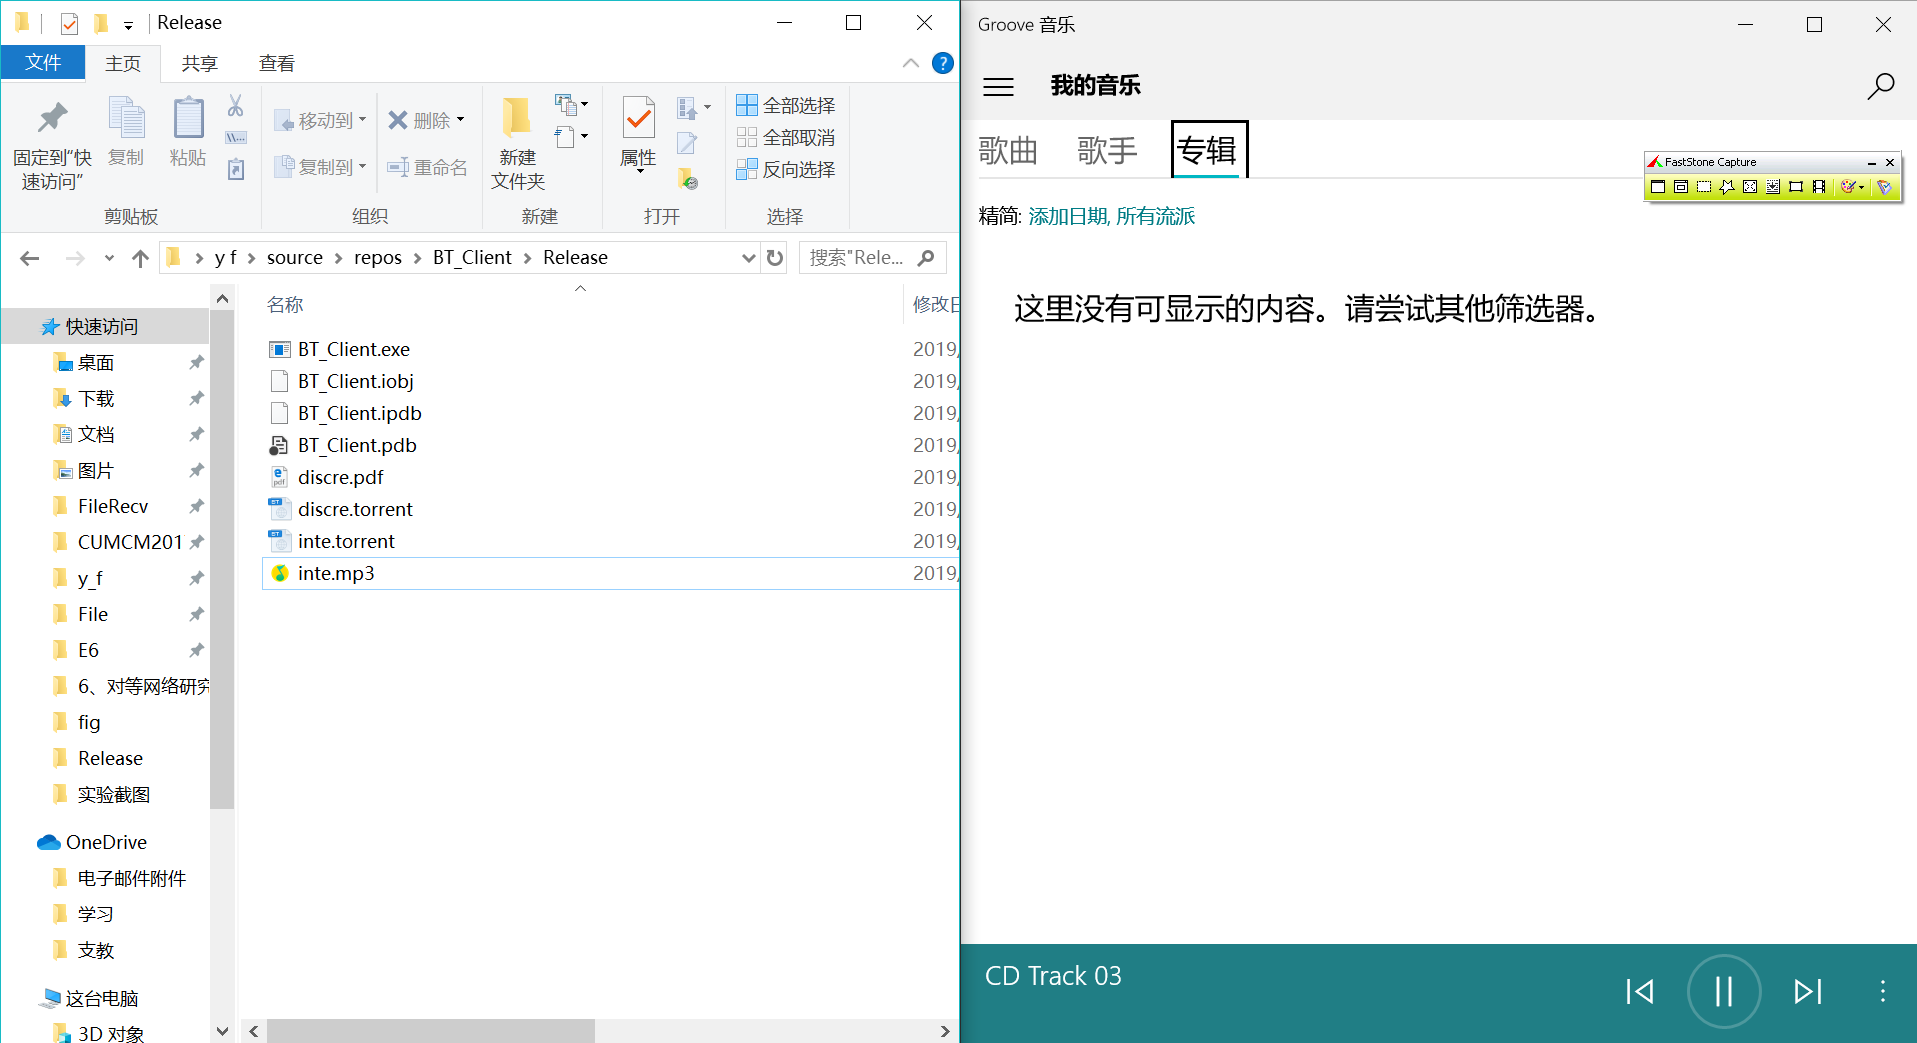
\includegraphics[width=0.45\linewidth]{fig/PC4_f2.png}
		}
		\caption{PC2发布的文件和PC}
		\label{res:file}		
	\end{figure}

	\subsection{1-3实验}
	接下来我们尝试了1个下载者向3个拥有者下载文件。PC1作为服务器(图\ref{res:PC1_31})。PC2(图\ref{res:PC2_31})、3(图\ref{res:PC3_31})、5(图\ref{res:PC5_31})作为文件发布者。PC4从三个文件拥有者处下载文件(图\ref{res:PC4_31})。1-3实验网络拓扑结构图如\ref{res:13}所示。

	\begin{figure}[H]
		\centering
		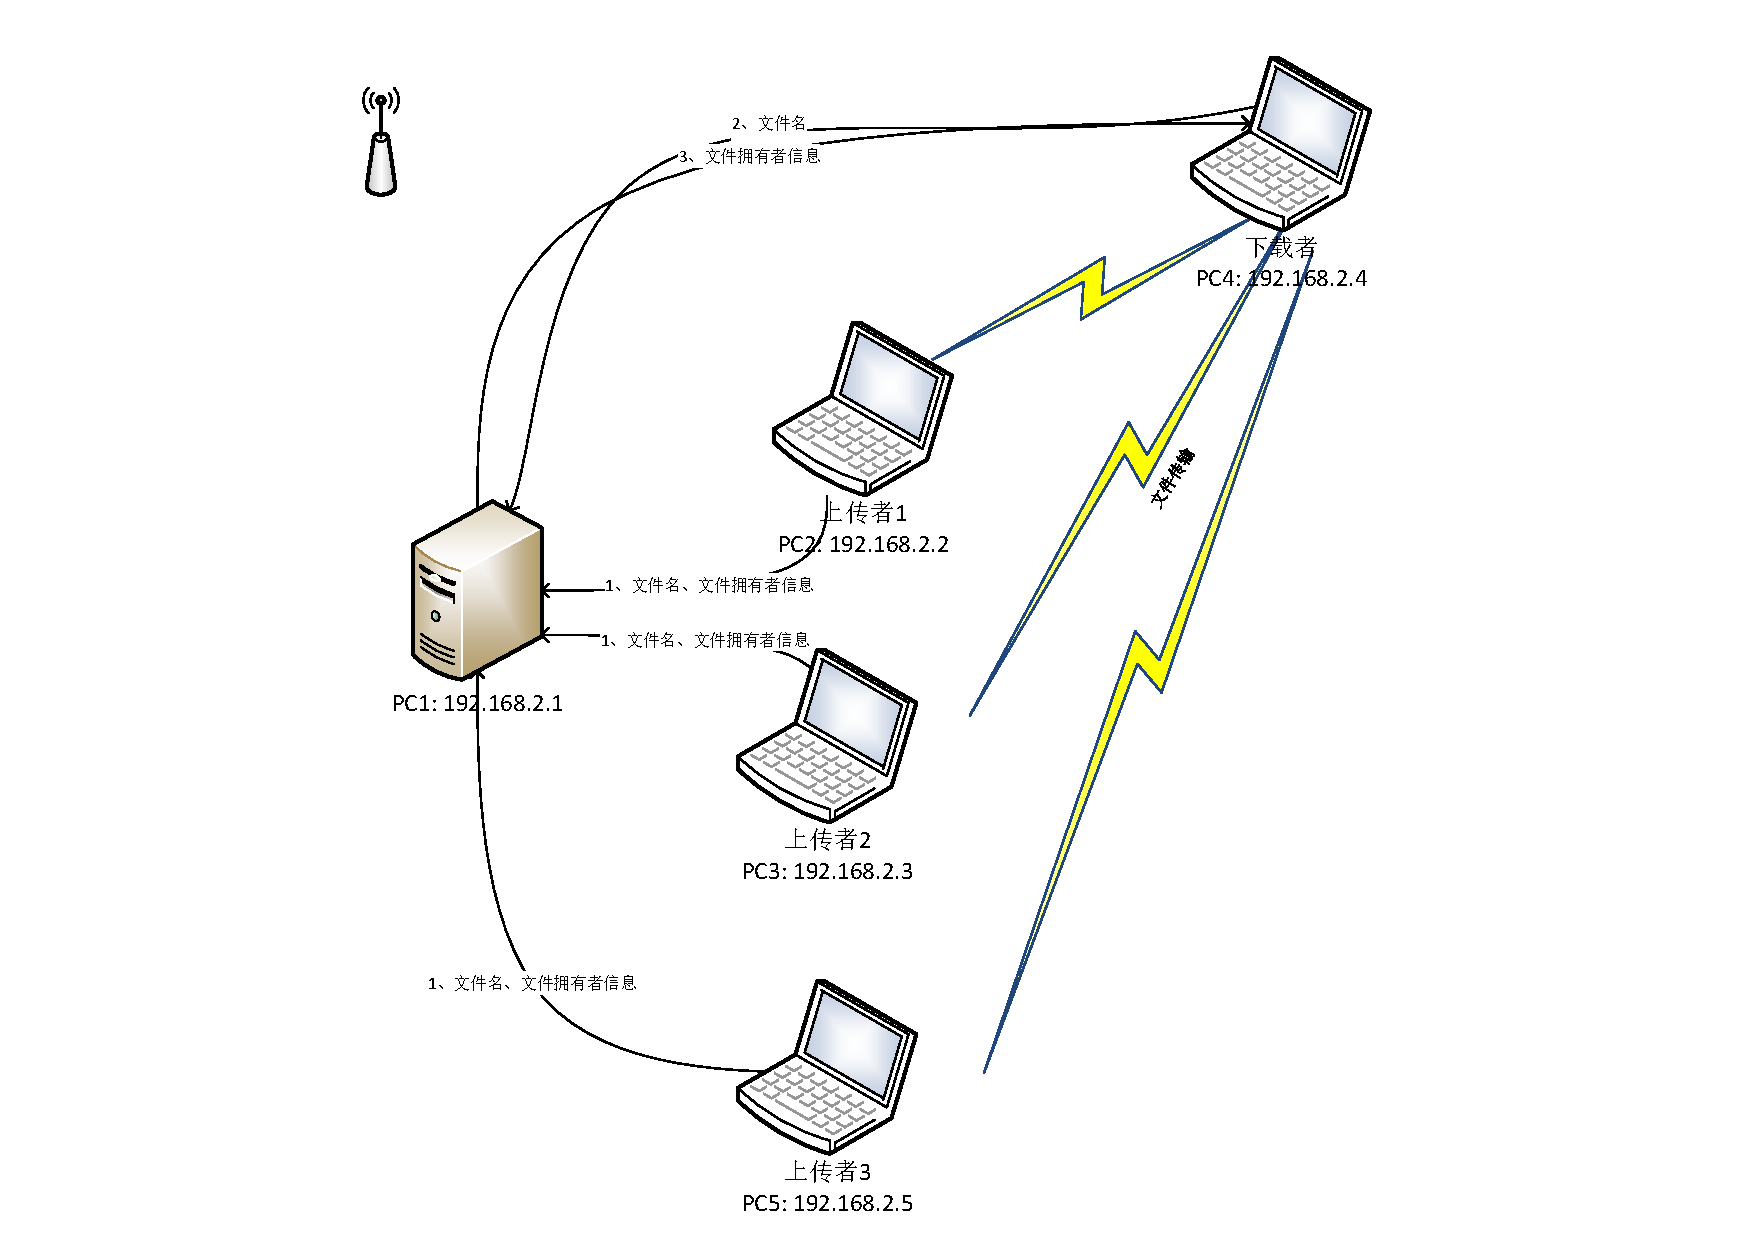
\includegraphics[width=0.8\linewidth]{fig/3-1.pdf}
		\caption{1-3实验\quad 网络拓扑结构图}
		\label{res:13}
	\end{figure}
	\begin{minipage}{0.5\linewidth}
	\begin{figure}[H]
		\centering
		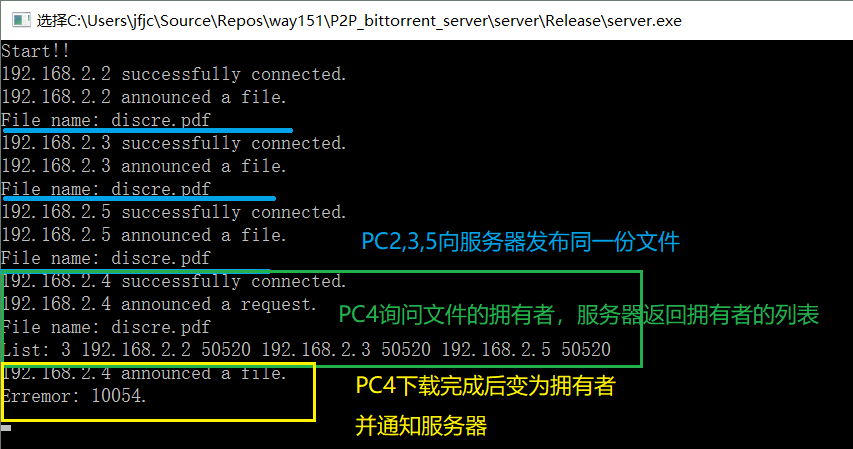
\includegraphics[width=\linewidth]{fig/PC1_31.png}
		\caption{1-3实验\quad PC1作为服务器}
		\label{res:PC1_31}
	\end{figure}
	\end{minipage}
	\begin{minipage}{0.5\linewidth}
	\begin{figure}[H]
		\centering
		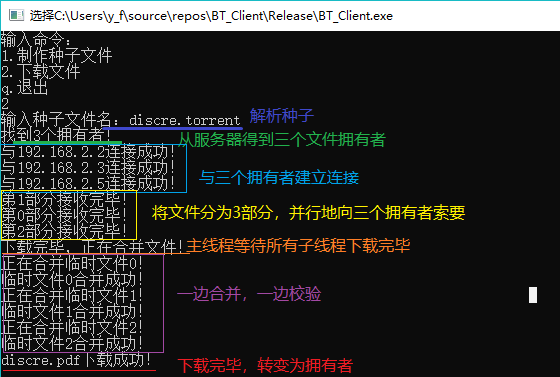
\includegraphics[width=\linewidth]{fig/PC4_31.png}
		\caption{1-3实验\quad PC4作为下载者}
		\label{res:PC4_31}
	\end{figure}
	\end{minipage}
	\begin{minipage}{0.5\linewidth}
	\begin{figure}[H]
		\centering
		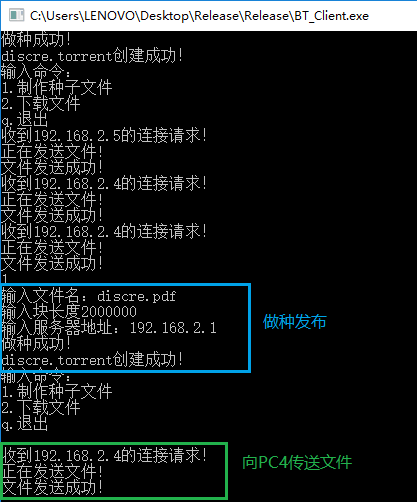
\includegraphics[width=\linewidth]{fig/PC2_31.png}
		\caption{1-3实验\quad PC2作为文件发布者}
		\label{res:PC2_31}
	\end{figure}
	\end{minipage}
	\begin{minipage}{0.5\linewidth}
	\begin{figure}[H]
		\centering
		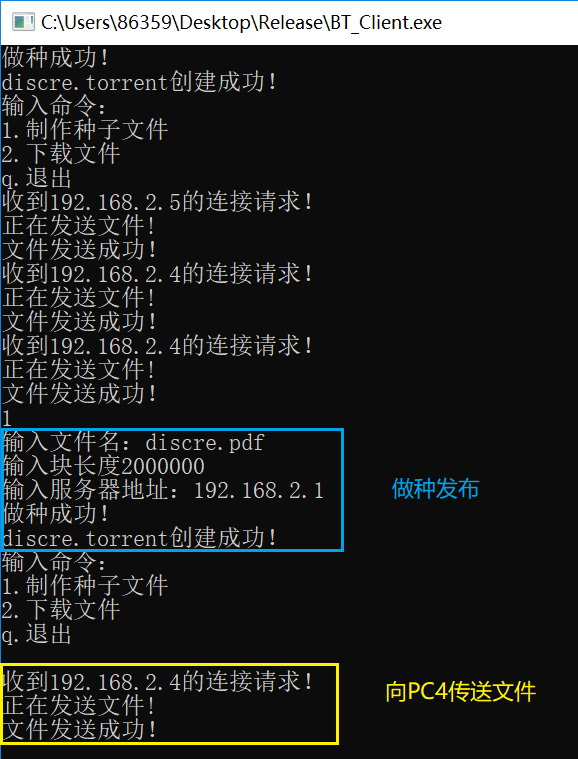
\includegraphics[width=0.9\linewidth]{fig/PC3_31.png}
		\caption{1-3实验\quad PC3作为文件发布者}
		\label{res:PC3_31}
	\end{figure}
	\end{minipage}
	\begin{figure}[H]
		\centering
		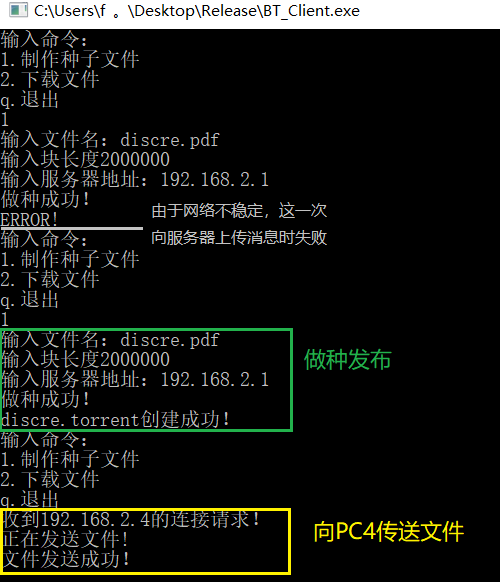
\includegraphics[width=0.4\linewidth]{fig/PC5_31.png}
		\caption{1-3实验\quad PC5作为文件发布者}
		\label{res:PC5_31}
	\end{figure}
	

	\subsection{2-1实验}
	这一步尝试2个下载者同时从1个拥有者处下载文件。PC1作为服务器(图\ref{res:PC1_12})。PC2作为文件发布者(图\ref{res:PC2_12})。PC3(图\ref{res:PC3_12}),4(图\ref{res:PC4_12})从PC2处下载文件。2-1实验网络拓扑结构图如图\ref{res:21}所示
	\begin{figure}[H]
		\centering 
		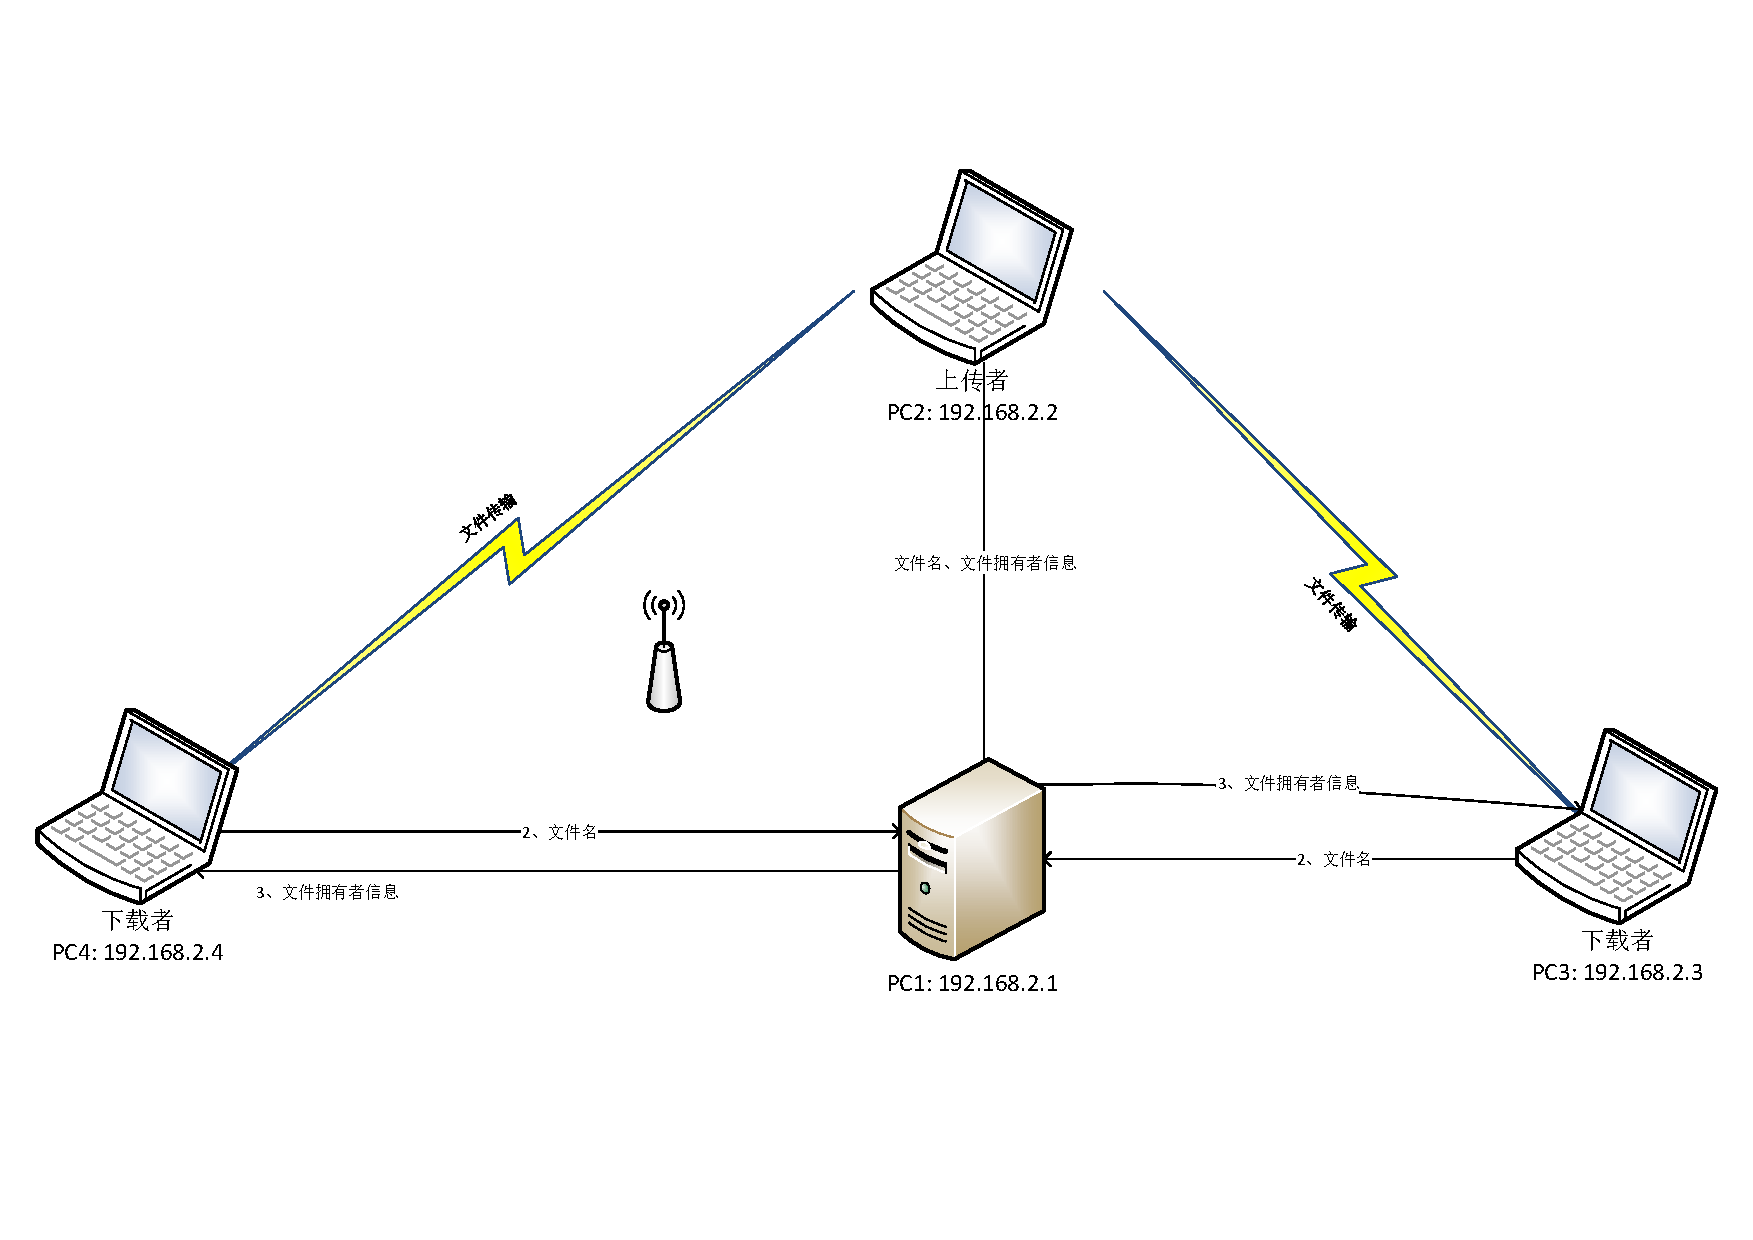
\includegraphics[width=0.6\linewidth]{fig/2-1.pdf}
		\caption{2-1实验\quad 网络拓扑结构图}
		\label{res:21}
	\end{figure}
	\begin{minipage}{0.5\linewidth}
	\begin{figure}[H]
		\centering
		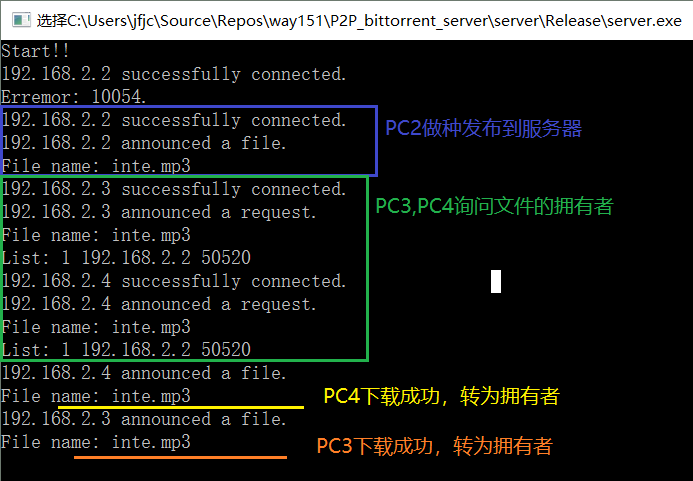
\includegraphics[width=\linewidth]{fig/PC1_12.png}
		\caption{2-1实验\quad PC1作为服务器}
		\label{res:PC1_12}
	\end{figure}
	\end{minipage}
	\begin{minipage}{0.5\linewidth}
	\begin{figure}[H]
		\centering
		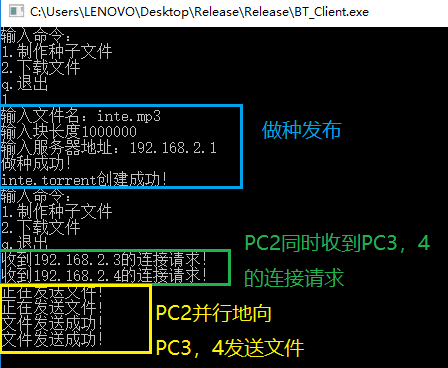
\includegraphics[width=\linewidth]{fig/PC2_12.png}
		\caption{2-1实验\quad PC2作为文件发布者}
		\label{res:PC2_12}
	\end{figure}
	\end{minipage}
	\begin{minipage}{0.5\linewidth}
	\begin{figure}[H]
		\centering
		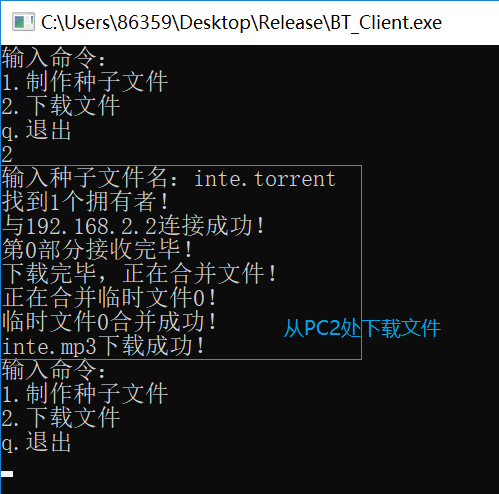
\includegraphics[width=0.9\linewidth]{fig/PC3_12.png}
		\caption{2-1实验\quad PC3作为下载者}
		\label{res:PC3_12}
	\end{figure}
	\end{minipage}
	\begin{minipage}{0.5\linewidth}
	\begin{figure}[H]
		\centering
		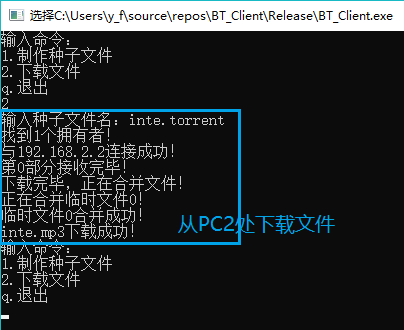
\includegraphics[width=\linewidth]{fig/PC4_12.png}
		\caption{2-1实验\quad PC4作为下载者}
		\label{res:PC4_12}
	\end{figure}
	\end{minipage}
	
	\subsection{2-2实验}
	最后我们尝试了多个下载者,多个文件拥有者之间传输文件。PC1作为服务器(图\ref{res:PC1_22})。PC2首先发布一份文件(图\ref{res:PC2_22}),然后PC3从PC2处下载。PC3下载完之后就变为了文件拥有者(图\ref{res:PC3_22})。之后PC4(图\ref{res:PC4_22}),5(图\ref{res:PC5_22})同时从PC2,3处下载文件。2-2实验网络拓扑结构图如图\ref{res:22}所示
	\begin{figure}[H]
		\centering
		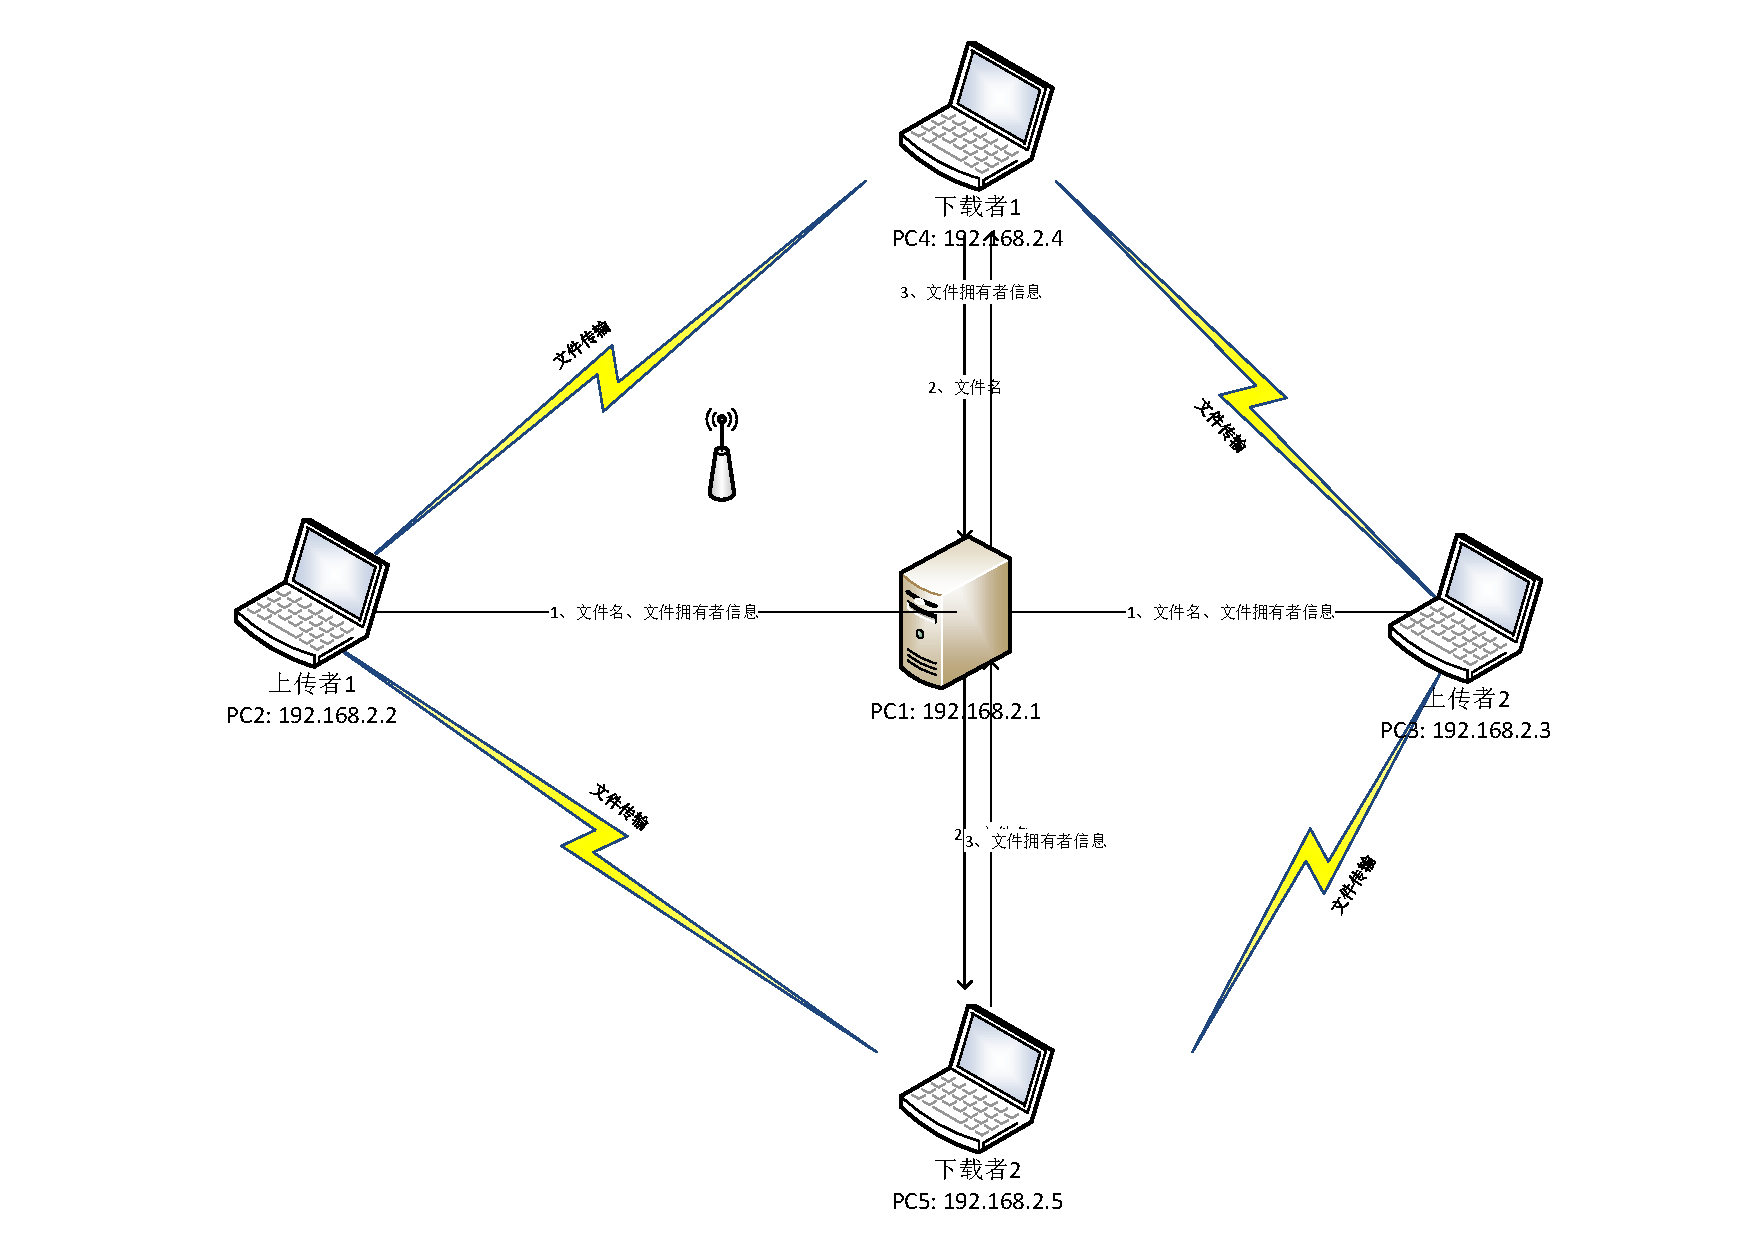
\includegraphics[width=0.8\linewidth]{fig/2-2.pdf}
		\caption{2-2实验\quad 网络拓扑结构图}
		\label{res:22}
	\end{figure}
	\begin{minipage}{0.5\linewidth}
	\begin{figure}[H]
		\centering
		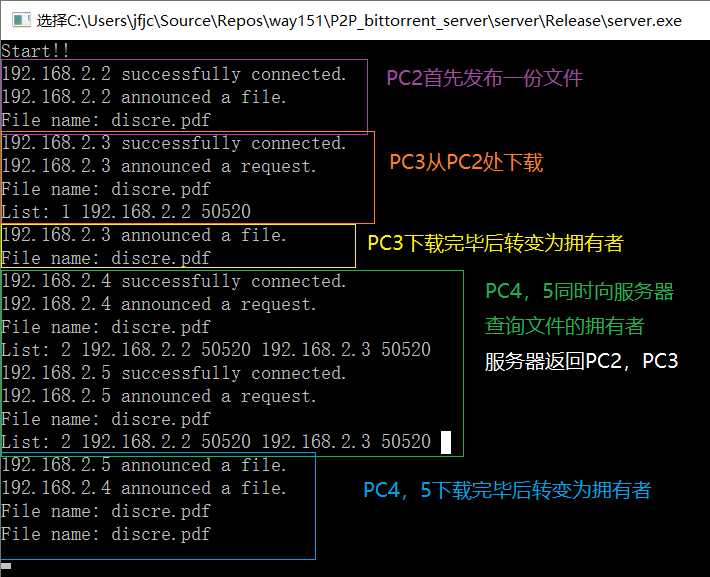
\includegraphics[width=\linewidth]{fig/PC1_22.png}
		\caption{2-2实验\quad PC1作为服务器}
		\label{res:PC1_22}
	\end{figure}
	\end{minipage}
	\begin{minipage}{0.5\linewidth}
	\begin{figure}[H]
		\centering
		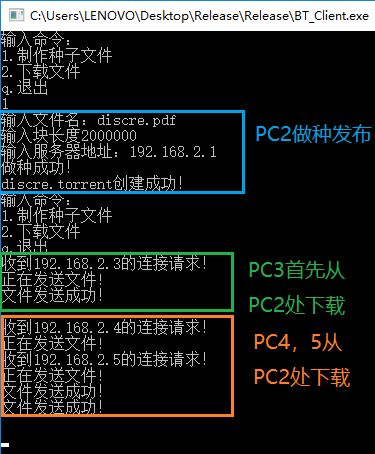
\includegraphics[width=\linewidth]{fig/PC2_22.png}
		\caption{2-2实验\quad PC2作为第一个文件发布者}
		\label{res:PC2_22}
	\end{figure}
	\end{minipage}
	\begin{minipage}{0.5\linewidth}
	\begin{figure}[H]
		\centering
		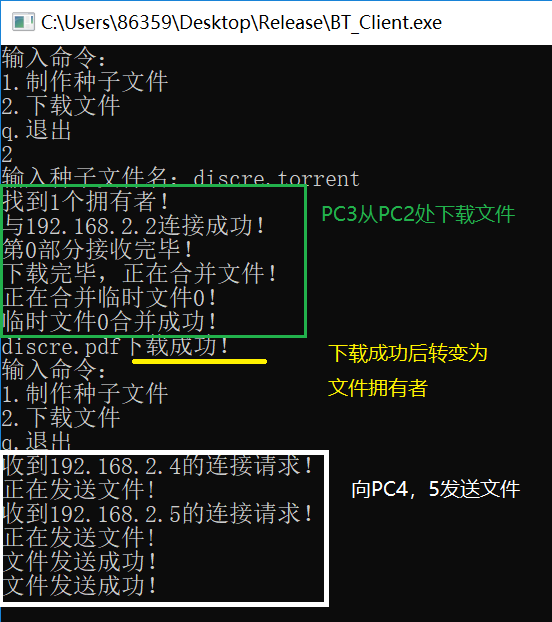
\includegraphics[width=\linewidth]{fig/PC3_22.png}
		\caption{2-2实验\quad PC3首先作为下载者,PC2处下载文件;下载成功后变为文件拥有者向PC4,5发送文件}
		\label{res:PC3_22}
	\end{figure}
	\end{minipage}
	\begin{minipage}{0.5\linewidth}
	\begin{figure}[H]
		\centering
		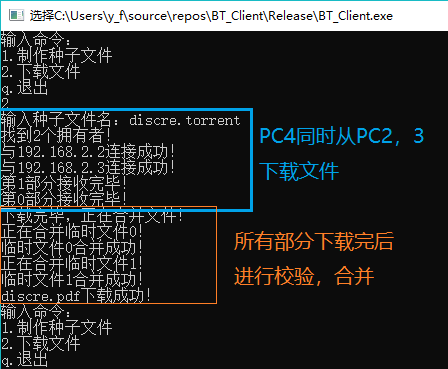
\includegraphics[width=\linewidth]{fig/PC4_22.png}
		\caption{2-2实验\quad PC4作为下载者}
		\label{res:PC4_22}
	\end{figure}
	\end{minipage}
	\begin{figure}[H]
		\centering
		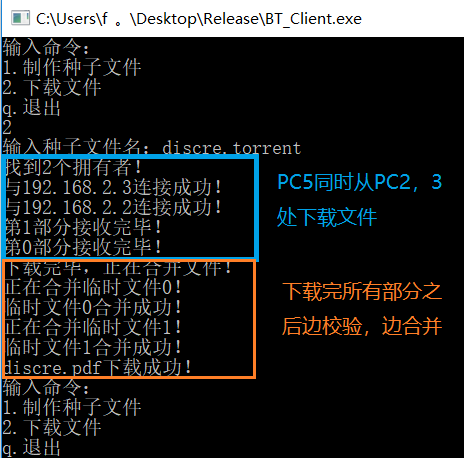
\includegraphics[width=0.4\linewidth]{fig/PC5_22.png}
		\caption{2-2实验\quad P52作为下载者}
		\label{res:PC5_22}
	\end{figure}
	
	\section{总结}
	本文简要介绍了对等网络的特点,并以BitTorrent协议为例进行深入研究。
	通过对BitTorrent协议文档的整理,阐述该协议的一些基本概念以及工作原理。
	同时给出具体的实现方法,并进行了详尽的实验分析,给后面的研究者提供了一定的参考。
	
	\bibliographystyle{unsrt}
	\bibliography{reference}
	
\end{document}

% 对等网络(P2P)研究(选做)
% (自己定题目)
% 实验目标:研究某种对等网络算法。
% 实验要求:所有资料都可以来自网络和参考书籍,要把算法描述清楚,不用改进算法。
% 内容参考:
% 1、P2P(对等网)的概念
% 2、P2P算法分类
% 3、P2P的主要算法的简要介绍
% 4、P2P实现的主要问题,例如、NAT穿透问题和解决方法
% 5、详细分析某个P2P的算法。详细到什么程度,自己定,可以采用举例的方式,主要是让别人容易看懂。
% 6、该P2P算法的实现和改进
% 格式参考:参考给出的一篇中文论文,参考文献可以给出网址,依贡献次序给出论文作者(学号姓名),也可以在第一页下方具体说明每个人的工作。

% 组队人数:1~6人,可以跨班

% 提交文件:课程论文(论文名.pdf) (长短不限,讲清楚就可以)
% 课程PPT(论文名.ppt) (讲解算法用)
% 源代码(论文名.rar)
% 提交地址:http://172.18.187.9/NetDisk/Default.aspx?vm=17net
%          实验上交/编程实验
% 截止日期:2019年6月18日 23:00 (周二)